% VLDB template version of 2020-08-03 enhances the ACM template, version 1.7.0:
% https://www.acm.org/publications/proceedings-template
% The ACM Latex guide provides further information about the ACM template

%\documentclass[sigconf,twocolumn]{acmart}
\documentclass[sigconf,twocolumn,nonacm,dvipsnames]{acmart}



% Authors, replace the red X's with your assigned DOI string during the rightsreview eform process.

\settopmatter{printacmref=true}
\usepackage{fancyhdr}
\usepackage{appendix}
\usepackage{paralist}
\usepackage{subcaption}
\usepackage{standalone}
\usepackage{color, colortbl}
\usepackage{listings}
\usepackage{scalerel}
\usepackage{tikz}
\usetikzlibrary{trees}
\usepackage{amsmath}
% \usepackage{amssymb}
\usepackage{pifont}
\usepackage[framemethod=TikZ]{mdframed}
\usepackage[capitalize,noabbrev]{cleveref}
\usepackage{enumitem}
\usepackage{xspace}

\usepackage{multicol}
\usepackage{multirow}
\usepackage{array}
\usepackage{rotating}
% \usepackage{xcolor}
\usepackage{makecell}
\usepackage{xspace}
\definecolor{vlightgray}{gray}{0.85}
\def\pvt{PVT\xspace}
\newcommand{\turnrow}{\footnotesize\rotatebox{90}}
\newcommand{\maxlen}{\textsc{LenBound}\xspace}
\newcommand{\bound}{\textsc{Bound}\xspace}
\newcommand{\domain}{\textsc{Domain}\xspace}
\newcommand{\datasize}{\textsc{DataSize}\xspace}
\newcommand{\cc}{\textsc{ConfCons}\xspace}
\newcommand{\functional}{\textsc{Functional}\xspace}
\newcommand{\correlation}{\textsc{Indep}\xspace}
\newcommand{\regex}{\textsc{RegEx}\xspace}
\newcommand{\dependency}{\textsc{Causes}\xspace}
\newcommand{\condind}{\textsc{CondIndep}\xspace}
\newcommand{\attributeorder}{\textsc{AttributeOrder}\xspace}
\newcommand{\schema}{\textsc{SemanticType}\xspace}
\newcommand{\outlier}{\textsc{Outlier}\xspace}
\newcommand{\selectivity}{\textsc{Selectivity}\xspace}
\newcommand{\missing}{\textsc{Missing}\xspace}
\newcommand{\pplfail}{$\mathit{People_{fail}}$\xspace}
\newcommand{\pplpass}{$\mathit{People_\mathit{pass}}$\xspace}
\newcommand{\coverage}{\ensuremath{\textsc{Coverage}}}

% \usepackage[table,xcdraw]{xcolor}
\usepackage{arydshln}

\newcommand{\fairnessconstraints}{{\ensuremath{\mathcal F}}}
\newcommand{\coverageconstraints}{{\ensuremath{\mathcal C}}}
\newcommand{\mutable}{{\ensuremath{\mathbf M}}}
\newcommand{\immutable}{{\ensuremath{\mathbf I}}}
\newcommand{\patterngroup}{\ensuremath{\pattern_{{\tt grp}}}}
\newcommand{\patterninterv}{\ensuremath{\pattern_{{\tt int}}}}

\Crefname{algocf}{Algorithm}{Algorithms}
\usepackage[colorinlistoftodos]{todonotes}
\newcommand{\srtodo}[1]{{\reversemarginpar \todo[nolist]{{\tiny sr: #1}}}}

% \lstset{
% % numbers=left, 
% % numberstyle=\small, 
% % numbersep=8pt, 
% frame = single, 
% % language=Pascal, 
% % framexleftmargin=0pt
% }

\newcommand{\paratitle}[1]{
% \vspace{1mm} 
\noindent{\bf #1.}}

\captionsetup[figure]{skip=0pt}
\setlength{\abovedisplayskip}{0pt}
\setlength{\belowdisplayskip}{0pt}
\setlength{\abovecaptionskip}{0pt}
\setlength{\belowcaptionskip}{0pt}
\setlength{\textfloatsep}{1pt} %actually works to reduce 



\newcommand{\xmark}{\ding{55}}%

\lstset{
frame = single, 
  basicstyle=\ttfamily,
  columns=fullflexible,
%   keepspaces=true,
}

% \usepackage[font={small}]{caption}

% \pagenumbering{gobble}

% \usepackage[noend]{algpseudocode}
% \usepackage{algorithmicx,algorithm}
\usepackage[vlined,commentsnumbered,ruled]{algorithm2e}%,linesnumbered
\let\oldnl\nl% Store \nl in \oldnl
\newcommand{\nonl}{\renewcommand{\nl}{\let\nl\oldnl}}% Remove line number for one line
% \usepackage{bbm}
\newcommand\mycommfont[1]{\footnotesize\ttfamily\textcolor{blue}{#1}}
\SetCommentSty{mycommfont}




\def\HiLi{\leavevmode\rlap{\hbox to \hsize{\color{red!20}\leaders\hrule height .8\baselineskip depth .5ex\hfill}}}

\newcommand\new[1]{\textcolor{blue}{#1}\xspace}
\newcommand\independent{\protect\mathpalette{\protect\independenT}{\perp}}
\def\independenT#1#2{\mathrel{\rlap{$#1#2$}\mkern2mu{#1#2}}}

\usepackage{amsfonts}
\usepackage{amsmath}
\usepackage{comment}
\usepackage{multirow}
\usepackage{paralist}
\usepackage{paralist}
\usepackage{mathtools}
% \usepackage{amsmath,amssymb}
% \usepackage{todonotes}
\usepackage{framed}

%\usepackage[a4paper, margin=0.01cm]{geometry} 

\newtheorem{problem}{Problem}
% Comment out [section] to remove section number dependence
%\theoremstyle{definition}
\newtheorem{definition}{Definition}[section]
\newtheorem{theorem}{Theorem}[section]

\newtheorem{example}{Example}[section]
\newtheorem{solution}{Solution}[section]
\newtheorem{issue}{Issue}[section]
\newtheorem{query}{Query}[section]
\newtheorem{observation}{Observation}[section]


\newcommand{\AlignLeft}{\hspace*{\parindent}\hspace*{-\mathindent}}
\newcommand{\sr}[1]{\textcolor{purple}{\bf (SR:)~[#1]}{\typeout{#1}}}
\newcommand{\sg}[1]{\textcolor{red}{\bf (Sainyam)~[#1]}
{\typeout{#1}}}
\newcommand{\brit}[1]{\textcolor{teal}{\bf (Brit)~[#1]}{\typeout{#1}}}
\newcommand{\nativ}[1]{\textcolor{magenta}{\bf (Nativ)~[#1]}{\typeout{#1}}}
\newcommand{\ignore}[1]{}
\DeclareMathOperator*{\argmax}{arg\,max}

\newcommand{\blue}[1]{{\color{blue} {#1}}}

\newcommand{\red}[1]{{\color{red} {#1}}}

\newcommand{\newtext}[1]{{\color{cyan} {#1}}}
\newcommand{\newtextold}[1]{{#1}}
\newcommand{\magenta}[1]{{\color{magenta} {#1}}}

\newcommand{\cut}[1]{}

% MACROS
\newcommand{\probName}{Prescription Ruleset Selection}
\newcommand{\algoName}{\textsc{algo-name}}
\newcommand{\sysName}{\textsc{FairCap}\xspace}
\newcommand{\attrset}{\ensuremath{\mathbb{A}}}
\newcommand{\attrsubset}{\ensuremath{\mathcal{A}_{gb}}}
\newcommand{\dom}{{\tt dom}}
\newcommand{\varset}{\ensuremath{\mathbb{V}}}
\newcommand{\doop}{{\tt do}}
\newcommand{\db}{\ensuremath{D}}
\newcommand{\Qagg}{\ensuremath{Q}}
\newcommand{\gr}{g}
\newcommand{\causalG}{\ensuremath{G}}
\newcommand{\exo}{\ensuremath{\mathbf{U}}}
% \newcommand{\endovar}{\ensuremath{\mathcal{N}}}
\newcommand{\pattern}{\ensuremath{\mathcal{P}}}
\newcommand{\model}{\ensuremath{\mathcal{G}_\db}}
\newcommand{\edvar}{\ensuremath{\mathbf{V}}}



% \usepackage{xcolor}
% \usepackage{amsmath,amssymb}
% \usepackage{todonotes}
\definecolor{moonstoneblue}{rgb}{0.45, 0.66, 0.76}
\definecolor{oldlace}{rgb}{0.99, 0.96, 0.9}
\definecolor{mintcream}{rgb}{0.96, 1.0, 0.98}
\definecolor{mintgreen}{rgb}{0.0, 0.5, 0.0}
\definecolor{mistyrose}{rgb}{1.0, 0.89, 0.88}
\definecolor{palegold}{rgb}{0.9, 0.75, 0.54}
\definecolor{palechestnut}{rgb}{0.87, 0.68, 0.69}


\newcommand{\lastday}[1]{{\leavevmode\color{black}{#1}}}

\newcommand{\reva}[1]{{\leavevmode\color{black}{#1}}}
\newcommand{\revb}[1]{{\leavevmode\color{black}{#1}}}
% \newcommand{\revc}[1]{\textcolor{RedOrange}{#1}}
% \newcommand{\revc}[1]{{\leavevmode\color{purple}{#1}}}
\newcommand{\revc}[1]{{\leavevmode\color{black}{#1}}}
% \newcommand{\common}[1]{\textcolor{Bittersweet}{#1}}
\newcommand{\common}[1]{{\leavevmode\color{black}{#1}}}


\def\HiLiG{\leavevmode\rlap{\hbox to \hsize{\color{green!30}\leaders\hrule height .8\baselineskip depth .5ex\hfill}}}
\def\HiLiY{\leavevmode\rlap{\hbox to \hsize{\color{yellow!50}\leaders\hrule height .8\baselineskip depth .5ex\hfill}}}
\usepackage{wrapfig}
\definecolor{light-gray}{gray}{0.95}
\usepackage{tcolorbox}

\usepackage{tikz}
\newcommand*\circled[1]{\tikz[baseline=(char.base)]{
            \node[shape=circle,draw,inner sep=2pt] (char) {#1};}}
\tcbuselibrary{breakable}

\definecolor{darkgreen}{RGB}{0, 200, 0}
\definecolor{experimentblue}{RGB}{127, 159, 186}
\definecolor{experimentgreen}{RGB}{127, 186, 130}
\definecolor{experimentred}{RGB}{186, 138, 127}
\definecolor{experimentgray}{RGB}{94,94,94}

\newtcolorbox[auto counter,number within=subsection]{ruleset}[1]{
  breakable, boxrule=0pt, boxsep=3pt,left=0pt,right=0pt,top=0pt,bottom=0pt,  colback=white, colframe=black,colbacktitle=experimentgray, title=#1:,
}

\newtcolorbox[auto counter,number within=subsection]{summary}[1]{
  breakable, boxrule=0pt, boxsep=3pt,left=0pt,right=0pt,top=0pt,bottom=0pt, colbacktitle=experimentgreen, title=#1:,
}


\newcommand{\tabincell}[2]{\begin{tabular}{@{}#1@{}}#2\end{tabular}}
% \newcommand\independent{\protect\mathpalette{\protect\independenT}{\perp}}
\def\independenT#1#2{\mathrel{\rlap{$#1#2$}\mkern2mu{#1#2}}}


\settopmatter{printacmref=false}

\settopmatter{printfolios=true} % add page numbers

\setlength{\abovedisplayskip}{0pt}
\setlength{\belowdisplayskip}{0pt}
\setlength{\abovedisplayshortskip}{0pt}
\setlength{\belowdisplayshortskip}{0pt}


\begin{document}

% \begin{figure*}[h!]
\centering
{\sffamily
\textbf{Component:} Ibitech 57 coated Normalausführung 2 mm weiss\\
(Woven polypropylene)
}
\begin{tabular}{p{7cm} p{7cm}}
\begin{custommdframed}

\textbf{With Datasheet Context}
\vspace{0.5em}

Activity name: Polyester film production, coating 

Activity information: 

Polyethylene terephthalate (PET) film coated with a polyester-based material, assumed to be the product of a process that transforms ethylene glycol and terephthalic acid into PET and then coats it. Transformation process of transforming ethylene glycol and terephthalic acid into polyethylene terephthalate (PET) and applying a coating.
\end{custommdframed}
 & 
\begin{custommdframed}
\centering
\textbf{Without Datasheet Context}
\vspace{0.5em}

 Activity name: Polypropylene production, film or sheet

Activity information: 

Synthetic fibres-based non-woven with a polypropylene scrim coating, assumed to consist of 50\% synthetic fibers, 35\% synthetic resin, and 15\% polypropylene textile reinforcement. The transformation process includes the application of a synthetic resin in a water dispersion onto a base material consisting of synthetic fibers and a polypropylene scrim.
Transformation process includes non-woven production and coating process with a polypropylene production as precursor for the scrim component.
\end{custommdframed}
\end{tabular}
\label{response}
\caption{Sample LLM response for a BOM component. Inclusion of datasheet context appears to considerably improve reliability of responses.}
\end{figure*}


\title{Fair and Actionable Causal Prescription Ruleset}




\author{Benton Li}
\affiliation{%
  \institution{Cornell University}
  \country{USA}
}
\email{cl2597@cornell.edu}

\author{Nativ Levy}
\affiliation{%
  \institution{Technion}
   \country{Israel}
}
\email{nativlevymail@gmail.com}

\author{Brit Youngmann}
\affiliation{%
  \institution{Technion}
   \country{Israel}
}
\email{brity@technion.ac.il}

\author{Sainyam Galhotra}
\affiliation{%
  \institution{Cornell University}
   \country{USA}
}
\email{sg@cs.cornell.edu}

\author{Sudeepa Roy}
\affiliation{%
  \institution{Duke University}
   \country{USA}
}
\email{sudeepa@cs.duke.edu}

%%
%% By default, the full list of authors will be used in the page
%% headers. Often, this list is too long, and will overlap
%% other information printed in the page headers. This command allows
%% the author to define a more concise list
%% of authors' names for this purpose.
\renewcommand{\shortauthors}{Li et al.}





\begin{abstract}

Prescriptions, or actionable recommendations, are commonly generated across various fields to influence key outcomes such as improving public health, enhancing economic policies, or increasing business efficiency. While traditional association-based methods may identify correlations, they often fail to reveal the underlying causal factors needed for informed decision-making. 
%They serve as a vital tool in decision-making by providing targeted interventions to optimize an outcome of interest.
On the other hand, in decision making for tasks with significant societal or economic impact, it is crucial to provide recommendations that are justifiable and equitable in terms of the outcome for both the protected and non-protected groups. 
%and justifiable to ensure informed, equitable outcomes.
Motivated by these two goals,  this paper introduces a fairness-aware framework leveraging causal reasoning for generating a set of actionable prescription rules (ruleset) toward betterment of an outcome while preventing exacerbating inequalities for protected groups.
%ensuring equitable treatment across diverse populations. 
%We leverage causal reasoning to \newtext{generate the prescriptions toward betterment of an outcome in the form of a set of rules (ruleset)} while incorporating fairness and coverage constraints to prevent exacerbating inequalities. 
By considering group and individual fairness metrics from the literature, we ensure that both protected and non-protected groups benefit from these recommendations, providing a balanced and equitable approach to decision-making. We employ efficient optimizations to explore the vast and complex search space considering both fairness and coverage of the ruleset. Empirical evaluation and case study on real-world datasets 
%varying fairness criteria 
demonstrates the utility 
%developed formulations 
of our framework for different use cases.
\end{abstract}



\maketitle

% %%% do not modify the following VLDB block %%
% %%% VLDB block start %%%
% \pagestyle{\vldbpagestyle}
% \begingroup\small\noindent\raggedright\textbf{PVLDB Reference Format:}\\
% \vldbauthors. \vldbtitle. PVLDB, \vldbvolume(\vldbissue): \vldbpages, \vldbyear.\\
% \href{https://doi.org/\vldbdoi}{doi:\vldbdoi}
% \endgroup
% \begingroup
% \renewcommand\thefootnote{}\footnote{\noindent
% This work is licensed under the Creative Commons BY-NC-ND 4.0 International License. Visit \url{https://creativecommons.org/licenses/by-nc-nd/4.0/} to view a copy of this license. For any use beyond those covered by this license, obtain permission by emailing \href{mailto:info@vldb.org}{info@vldb.org}. Copyright is held by the owner/author(s). Publication rights licensed to the VLDB Endowment. \\
% \raggedright Proceedings of the VLDB Endowment, Vol. \vldbvolume, No. \vldbissue\ %
% ISSN 2150-8097. \\
% \href{https://doi.org/\vldbdoi}{doi:\vldbdoi} \\
% }\addtocounter{footnote}{-1}\endgroup
% %%% VLDB block end %%%

% %%% do not modify the following VLDB block %%
% %%% VLDB block start %%%
% \ifdefempty{\vldbavailabilityurl}{}{
% \vspace{.3cm}
% \begingroup\small\noindent\raggedright\textbf{PVLDB Artifact Availability:}\\
% The source code, data, and/or other artifacts have been made available at \url{\vldbavailabilityurl}.
% \endgroup
% }
% %%% VLDB block end %%%


\section{Introduction}

Tutoring has long been recognized as one of the most effective methods for enhancing human learning outcomes and addressing educational disparities~\citep{hill2005effects}. 
By providing personalized guidance to students, intelligent tutoring systems (ITS) have proven to be nearly as effective as human tutors in fostering deep understanding and skill acquisition, with research showing comparable learning gains~\citep{vanlehn2011relative,rus2013recent}.
More recently, the advancement of large language models (LLMs) has offered unprecedented opportunities to replicate these benefits in tutoring agents~\citep{dan2023educhat,jin2024teach,chen2024empowering}, unlocking the enormous potential to solve knowledge-intensive tasks such as answering complex questions or clarifying concepts.


\begin{figure}[t!]
\centering
\includegraphics[width=1.0\linewidth]{Figs/Fig.intro.pdf}
\caption{An illustration of coding tutoring, where a tutor aims to proactively guide students toward completing a target coding task while adapting to students' varying levels of background knowledge. \vspace{-5pt}}
\label{fig:example}
\end{figure}

\begin{figure}[t!]
\centering
\includegraphics[width=1.0\linewidth]{Figs/Fig.scaling.pdf}
\caption{\textsc{Traver} with the trained verifier shows inference-time scaling for coding tutoring (detailed in \S\ref{sec:scaling_analysis}). \textbf{Left}: Performance vs. sampled candidate utterances per turn. \textbf{Right}: Performance vs. total tokens consumed per tutoring session. \vspace{-15pt}}
\label{fig:scale}
\end{figure}


Previous research has extensively explored tutoring in educational fields, including language learning~\cite{swartz2012intelligent,stasaski-etal-2020-cima}, math reasoning~\cite{demszky-hill-2023-ncte,macina-etal-2023-mathdial}, and scientific concept education~\cite{yuan-etal-2024-boosting,yang2024leveraging}. 
Most aim to enhance students' understanding of target knowledge by employing pedagogical strategies such as recommending exercises~\cite{deng2023towards} or selecting teaching examples~\cite{ross-andreas-2024-toward}. 
However, these approaches fall short in broader situations requiring both understanding and practical application of specific pieces of knowledge to solve real-world, goal-driven problems. 
Such scenarios demand tutors to proactively guide people toward completing targeted tasks (e.g., coding).
Furthermore, the tutoring outcomes are challenging to assess since targeted tasks can often be completed by open-ended solutions.



To bridge this gap, we introduce \textbf{coding tutoring}, a promising yet underexplored task for LLM agents.
As illustrated in Figure~\ref{fig:example}, the tutor is provided with a target coding task and task-specific knowledge (e.g., cross-file dependencies and reference solutions), while the student is given only the coding task. The tutor does not know the student's prior knowledge about the task.
Coding tutoring requires the tutor to proactively guide the student toward completing the target task through dialogue.
This is inherently a goal-oriented process where tutors guide students using task-specific knowledge to achieve predefined objectives. 
Effective tutoring requires personalization, as tutors must adapt their guidance and communication style to students with varying levels of prior knowledge. 


Developing effective tutoring agents is challenging because off-the-shelf LLMs lack grounding to task-specific knowledge and interaction context.
Specifically, tutoring requires \textit{epistemic grounding}~\citep{tsai2016concept}, where domain expertise and assessment can vary significantly, and \textit{communicative grounding}~\citep{chai2018language}, necessary for proactively adapting communications to students' current knowledge.
To address these challenges, we propose the \textbf{Tra}ce-and-\textbf{Ver}ify (\textbf{\model}) agent workflow for building effective LLM-powered coding tutors. 
Leveraging knowledge tracing (KT)~\citep{corbett1994knowledge,scarlatos2024exploring}, \model explicitly estimates a student's knowledge state at each turn, which drives the tutor agents to adapt their language to fill the gaps in task-specific knowledge during utterance generation. 
Drawing inspiration from value-guided search mechanisms~\citep{lightman2023let,wang2024math,zhang2024rest}, \model incorporates a turn-by-turn reward model as a verifier to rank candidate utterances. 
By sampling more candidate tutor utterances during inference (see Figure~\ref{fig:scale}), \model ensures the selection of optimal utterances that prioritize goal-driven guidance and advance the tutoring progression effectively. 
Furthermore, we present \textbf{Di}alogue for \textbf{C}oding \textbf{T}utoring (\textbf{\eval}), an automatic protocol designed to assess the performance of tutoring agents. 
\eval employs code generation tests and simulated students with varying levels of programming expertise for evaluation. While human evaluation remains the gold standard for assessing tutoring agents, its reliance on time-intensive and costly processes often hinders rapid iteration during development. 
By leveraging simulated students, \eval serves as an efficient and scalable proxy, enabling reproducible assessments and accelerated agent improvement prior to final human validation. 



Through extensive experiments, we show that agents developed by \model consistently demonstrate higher success rates in guiding students to complete target coding tasks compared to baseline methods. We present detailed ablation studies, human evaluations, and an inference time scaling analysis, highlighting the transferability and scalability of our tutoring agent workflow.

\section{Related Work} \label{sec:related}

In this section, we discuss related work that has not been covered in previous sections.

\paragraph{Static resource analysis}
%
AARA is not the only approach for type-based resource analysis.
%
For example, there are approaches based on sized types~\cite{phd:Vasconcelos08,ICFP:AL17}, dependent types~\cite{LICS:LG11,POPL:LP13,POPL:RGG21}, refinement types~\cite{POPL:HVH20,POPL:CBG17,ESOP:CGA15,OOPSLA:WWC17},
recurrence extraction~\cite{POPL:KML20,ICFP:DLR15}, logical frameworks~\cite{POPL:NSG22,POPL:GNS24}, and annotated types~\cite{POPL:CW00,POPL:Danielsson08}.
%
None of the aforementioned type systems considered supporting heap-manipulating programs with Rust's borrow mechanisms.
%
Besides type systems, there are also static resource-analysis techniques based on
defunctionalization~\cite{ICFP:ALM15}, recurrence relations~\cite{JAR:AAG11,TACAS:AFR15,APLAS:FH14,PLDI:BCK20,POPL:KBC19,PLDI:KBB17},
term rewriting~\cite{RTA:AM13,TACAS:BEG14,IJCAR:FNH16,JAR:NEG13}, and
abstract interpretation~\cite{SAS:ZSG11,LPAR:BHH10,CAV:SZV14,kn:DHW07,misc:fbinfer20,SAS:AG12}.
%
Some of the aforementioned techniques work on imperative programs (e.g., C programs) with arrays,
such as C4B~\cite{PLDI:CHS15}, SPEED~\cite{POPL:GMC09}, COSTA~\cite{JAR:AAG11}, ICRA~\cite{PLDI:KBB17}, etc., but none of them considered exploiting Rust's borrow mechanisms in the design.
%
It would be interesting future research direction to investigate how different static resource-analysis techniques can benefit from Rust's safety guarantees.

% Automatic Amortized Resource Analysis(AARA) first presented by \cite{AARA-Linear}, enriched type system  with resource annotations for a first-order functional language, to derive linear upper bounds on the heap-memory usage of list via linear programming. Derivative works support non-linear worst-case upper bound, like polynomial \cite{AARA-Poly}, multivariate polynomial \cite{AARA-Poly-Multivar}, exponential \cite{AARA-Exp} and logarithmic \cite {AARA-Log}. AARA can also support features like higher-order functions \cite{AARA-HigherOrder}, algebraic data types \cite{AARA-ADT} and general recursive data types \cite{AARA-GeneralRecursive}. Original AARA method does not support imperative mutation, whereas our work features AARA mainly with it and Rust borrow mechanism. Compared with AARA derivative works, our formalization is currently limited to single variate linear upper bound, however in our view, our extension is orthogonal to other features. Therefore it can be easy, as future works, to support complex recursive data structures and various upper bounds in Rust resource analyzer.

\paragraph{Graded type system}
Graded types \cite{Granule} introduce a graded modality for associating types with elements from a resource algebra. 
%
A graded type system can account for program variables' exact usages, security levels, and potentials (conceptually). 
%
Graded types seem to provide a more general mechanism than AARA types to reason about more general resources. 
%
On the other hand, our work focuses on how Rust's borrow mechanisms can aid resource analysis and chooses AARA as the starting point because AARA admits efficient type inference via linear programming. 

\paragraph{Program verification for Rust}
%
RustBelt~\cite{RustBelt} pioneers a line of work to use semantic typing and separation logic to verify Rust programs with both safe and unsafe code.
%
% Stacked Borrow \cite{StackedBorrow} presents an operational semantics for memory accesses in Rust, and defines an aliasing discipline to cooperate raw pointers and borrows when verifying. 
%
RustHorn~\cite{RustHorn} uses prophecy variables to model the future values of mutable borrows and proposes an automatic verification algorithm based on constrained Horn clauses.
%
% Another approach is to leverage Rust type system, restricting on safe Rust with borrow mechanism. 
Aeneas~\cite{Aeneas}---which inspires our development of RABC and supports our prototype implementation---uses LLBC to translate Rust programs into equivalent pure functional programs via symbolic execution.
%
Such pure functional programs can be ported into theorem provers such as Coq and F* to enable verification of functional correctness.
%
Prusti~\cite{OOPSLA:AMP19} also leverages Rust's advanced type system to devise a modular and automated verification approach.
%
\citet{master:Engel21} proposed a method to verify user-provided asymptotic resource bounds in Prusti.
%
In contrast, our work focuses on the automatic inference of concrete resource bounds via a type system.
%
% Refinement types based method has also been applied to verification, like Flux \cite{Flux} proposing a liquid type system and RefinedRust \cite{RefinedRust} exploiting prophecy variables. Our work follows type system based approach and focuses on analysis instead of verification. We admits safe restriction of Rust from Stacked Borrow, resembling Aeneas working on borrow calculus, but unnecessarily translating to functional program, straightforward analyzing resource consumption. We also adopt prophecy variables to model mutable borrows.

% \todo{MAY DELETE THIS merging? might similar to static analysis, when coming across loop}
\section{Background on Causal Inference}
\label{sec:background-causal} 



 \newtextold{In this section, we 
 %formalize the notion of {\em Average Treatment Effect and understand the 
 review the basic concepts and key assumptions for inferring the effects of an intervention on the outcome on collected datasets without performing randomized controlled experiments. 
We use {\em Pearl's graphical causal model} for {\em observational causal analysis} \cite{pearl2009causal} to define these concepts.}


\par
\paratitle{Causal Inference and Causal DAGs} The primary goal of causal inference is to model causal dependencies between attributes and evaluate how changing one variable (referred to as intervention) would affect the other.
Pearl's Probabilistic Graphical Causal Model \cite{pearl2009causal} can be written as a tuple $(\exo, \edvar, Pr_{\exo}, \psi)$, where $\exo$ is a set of {\em exogenous} variables, $\Pr_{\exo}$ is the joint distribution of \exo, and $\edvar$ is a set of observed {\em endogenous variables}.
Here $\psi$ is a set of structural equations that encode dependencies among variables. The equation for $A \in \edvar$ takes the following form:
%that encode the dependencies among the variables.  These equations are of the form 
$$\psi_{A}: 
\dom(Pa_{\exo}(A)) {\times} \dom(Pa_{\edvar}(A)) \to \dom(A)$$
Here $Pa_{\exo}(A) {\subseteq} {\exo}$ and $Pa_{\edvar}(A) {\subseteq} \edvar \setminus \{A\}$ respectively denote the exogenous and endogenous parents of $A$. A causal relational model is associated with a directed acyclic graph ({\em causal DAG}) $G$, whose nodes are the endogenous variables $\edvar$ and there is a directed edge from $X$ to $O$ if  $X {\in} Pa_{\edvar}(O)$. The causal DAG obfuscates exogenous variables as they are unobserved. %Any given set of values for the exogenous variables completely determines the values of the endogenous variables by the structural equations (we do not need any known closed-form expressions of the structural equations in this work). 
The probability distribution $\Pr_{\exo}$ on exogenous variables $\exo$ induces a probability distribution  
on the endogenous variables $\edvar$ by the structural equations $\psi$.  A causal DAG can be constructed by a domain expert as in the above example, or using existing {\em causal discovery} algorithms~\cite{glymour2019review}. 



\begin{figure}
    \centering
    \small
    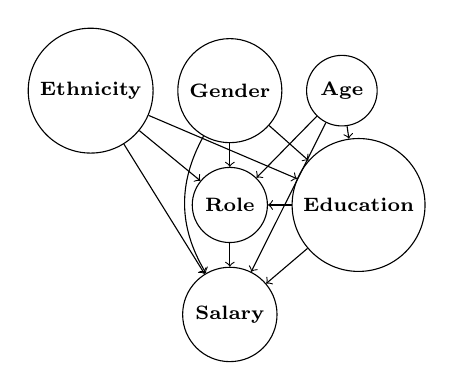
\begin{tikzpicture}[node distance=0.6cm and 1cm, every node/.style={minimum size=0.5cm}]
        \tikzset{vertex/.style = {draw, circle, align=center}}

        \node[vertex] (Ethnicity) {\bf\scriptsize{{Ethnicity}}};
        \node[vertex, right=0.3cm of Ethnicity] (Gender) {\bf{\scriptsize{Gender}}};
        \node[vertex, right=0.3cm of Gender] (Age) {\bf{\scriptsize{Age}}};
        \node[vertex, below=0.3cm of Gender] (Role) {\bf{\scriptsize{Role}}};
        \node[vertex, right=0.3cm of Role] (Education) {\bf{\small{\scriptsize{Education}}}};
        \node[vertex, below=0.3cm of Role] (Salary) {\bf{\scriptsize{Salary}}};

        \draw[->] (Ethnicity) -- (Salary);
        \draw[->] (Gender) -- (Role);
        \draw[->] (Age) -- (Role);
         \draw[->] (Education) -- (Role);
           \draw[->] (Education) -- (Salary);
             \draw[->] (Ethnicity) -- (Education);
                \draw[->] (Ethnicity) -- (Role);
             \draw[->] (Gender) -- (Education);
               \draw[->] (Age) -- (Education);
                 \draw[->] (Role) -- (Salary);
        \draw[->] (Gender) to[bend right] (Salary);
        \draw[->] (Age) -- (Salary);
    \end{tikzpicture}
    \caption{Partial causal DAG for the Stack Overflow dataset.}
    \label{fig:causal_DAG}
\end{figure}



 \begin{example}
Figure \ref{fig:causal_DAG} depicts a partial causal DAG for the SO dataset over the attributes in Table \ref{tab:data} as endogenous variables (we use a larger causal DAG with all 20 attributes in our experiments). 
  Given this causal DAG, we can observe that the role that a coder has in their company depends on their education, age gender and ethnicity.
\end{example}
\par


\par
\paratitle{Intervention} In Pearl's model, a treatment $T = t$ (on one or more variables) is considered as an {\em intervention} to a causal DAG by mechanically changing the DAG such that the values of node(s) of $T$ in $G$ are set to the value(s) in $t$, which is denoted by $\doop(T = t)$. Following this operation, the probability distribution of the nodes in the graph changes as the treatment nodes no longer depend on the values of their parents. Pearl's model gives an approach to estimate the new probability distribution by identifying the confounding factors $Z$ described earlier using conditions such as {\em d-separation} and {\em backdoor criteria} \cite{pearl2009causal}, which we do not discuss in this paper.


\par
\paratitle{Average Treatment Effect} The effects of an intervention are often measured by evaluating
% \par
% \paratitle{Causal inference, Treatment, ATE, and CATE}
% \newtextold{One of the primary goals  of {\em causal inference} is to estimate the effect of making a change in terms of a {\em treatment} $T$ (often referred to as an intervention)
% on the outcome $O$. 
% %A variable that is modified is often referred to as the treatment variable $T$ and the metric used to captures 
% The effect of treatment $T$ on outcome $O$ is measured by 
% %is known as 
{\em Conditional Average treatment effect (CATE)}, 
%a {\em treatment variable} $T$ on an outcome variable $O$ (e.g., what is the effect of higher \verb|Education| on \verb|Salary|). 
measuring the effect of an intervention on a subset of records~\cite{rubin1971use,holland1986statistics} by calculating the difference in average outcomes between the group that receives the treatment and the group that does not (called the {\em control} group), providing an estimate of how the intervention by $T$ influences an outcome $O$ for a given subpopulation. 
% Mathematically,
% \begin{equation}
%     %{\small ATE(T,O) = \mathbb{E}[O \mid \doop(T=1)] -      \mathbb{E}[O \mid \doop(T=0)]}
%     {\small ATE(T, O) = \mathbb{E}[O \mid \doop(T=1)] -  
%     \mathbb{E}[O \mid \doop(T=0)]}
% \label{eq:ate}
% \end{equation}
% In our work, where the treatment with maximum effect may vary among different subpopulations, we are interested in computing the \emph{Conditional Average Treatment Effect} (CATE), which measures the effect of a treatment on an outcome on \emph{a subset of input units}~\cite{rubin1971use,holland1986statistics}. 
Given a subset of the records defined by (a vector of) attributes $B$ and their values $b$, 
%g {\in} \Qagg(\db)$ defined by a predicate $G {=} g$ 
we can compute $CATE(T,O \mid B = b)$ as:
{
\begin{eqnarray}    
    %CATE(T,O \mid G=g) = \mathbb{E}[O \mid \doop(T=1)&, G=g] -  \mathbb{E}[O \mid \doop(T=0), G=g] 
   % CATE(T,O \mid B = b) = 
    \mathbb{E}[O \mid \doop(T=1), B = b] -  
    \mathbb{E}[O \mid \doop(T=0), B = b]\label{eq:cate}
\end{eqnarray}
}
Setting $B=\phi$ is equivalent to the ATE estimate.
The above definitions assumes that the treatment assigned to one unit does not affect the outcome of another unit (called the {Stable Unit Treatment Value Assumption (SUTVA)) \cite{rubin2005causal}}\footnote{This assumption does not hold for causal inference on multiple tables and even on a single table where tuples depend on each other.}. 


The ideal way of estimating the ATE and CATE is through {\em randomized controlled experiments}, 
where the population is randomly divided into two groups (treated and control, for binary treatments): 
%treated group that receives the treatment and control group that does not (denoted by 
%{the \em treated} group 
denoted by 
$\doop(T = 1)$ 
%for a binary treatment)  (the {\em control} group, 
and $\doop(T = 0)$ resp.)~\cite{pearl2009causal}.
%\sr{edited up to here, going to read the rest first, this section should not look like causumx}
%\par
%\par
However, randomized experiments cannot always be performed due to ethical or feasibility issues. In these scenarios, observational data is used to estimate the treatment effect, which requires the following additional assumptions. 
% {\em Observational Causal Analysis} still allows sound causal inference under additional assumptions. Randomization in controlled trials mitigates the effect of {\em confounding factors}, i.e., attributes that can affect the treatment assignment and outcome. Suppose we want to understand the causal effect of \verb|Education| on \verb|Salary| from the SO dataset.  %in Example~\ref{ex:running_example}. 
% We no longer apply Eq. (\ref{eq:ate}) since the values of \verb|Education| were not assigned at random in this data, and obtaining higher education largely depends on other attributes like \verb|Gender|, \verb|Age|, and \verb|Country|. 
% Pearl's model provides ways to account for these confounding attributes $Z$ to get an unbiased causal estimate from observational data under the following assumptions ($\independent$ denotes independence):
% \vspace{-2mm}
\newtextold{
The first assumption is called {\em unconfoundedness} or {\em strong ignorability}  \cite{rosenbaum1983central} says that the independence of outcome $O$ and treatment $T$ conditioning on a set of confounder variables  (covariates) $Z$, i.e.,
%\begin{eqnarray}
 $    O \independent T | Z {=} z$.
 %\label{eq:unconfoundedness}
%\end{eqnarray}
The second assumption called {\em overlap or positivity} says that there is a chance of observing individuals in both the treatment and control groups for every combination of covariate values, i.e., 
%\begin{eqnarray}
   $ 0 < Pr(T {=} 1 ~~|~~Z {=} z)< 1 $.
   %\label{eq:overlap}
%\end{eqnarray}
}
%\sg{Is this overlap or positivity? maybe both are the same?} \sr{yeah - same - from Google AI - The overlap assumption, also known as the positivity assumption, is a key assumption in causal inference that states that there is a chance of observing individuals in both the treatment and control groups for every combination of covariate values.}
% The above conditions are known as {\em Strong Ignorability} in Rubin's model \cite{rubin2005causal}.
The unconfoundedness assumption requires that the treatment $T$ and the outcome $O$ be independent when conditioned on a set of variables $Z$. In SO, assuming that only $Z$ =\{\verb|Gender|, \verb|Age|, \verb|Country|\} affects $T = $ \verb|Education|, if we condition on a fixed set of values of $Z$, i.e., consider people of a given gender, from a given country, and at a given age, then $T = $ \verb|Education| and $O = $ \verb|Salary| are independent. For such confounding factors $Z$,  Eq. (\ref{eq:cate}) reduces to the following form 
(positivity 
gives the feasibility of the expectation difference): 
 \vspace{-1mm}
{\small
\begin{flalign}    
% \begin{eqnarray}
   % % & ATE(T,O) = \mathbb{E}_Z \left[\mathbb{E}[O \mid T=1, Z = z] -  
   %  \mathbb{E}[O \mid T=0, Z = z] \right] \label{eq:conf-ate}\\
 & CATE(T,O {\mid} B {=} b) {=} \nonumber
    \mathbb{E}_Z \left[\mathbb{E}[O {\mid} T{=}1, B {=} b, Z {=} z] {-}  
    \mathbb{E}[O {\mid} T{=}0, B {=} b, Z {=} z]\right]\label{eq:conf-cate}
\end{flalign}
% \end{eqnarray}
}
% \vspace{-4mm}
This equation contains conditional probabilities and not $\doop(T = b)$, which can be estimated from an observed data. 
Pearl's model gives a systematic way to find such a $Z$ when a causal DAG is available. 




\subsection{Problem Formulation: Goal-State Conditioned Manipulation}
%\todo{Jane: I think we need to start with Imitation learning as in Hydra paper, given demo dataset of observation and actions }
\todo{Jane will work on this section - will propose to use notations at three levels per slack message}
Consider a robot manipulating objects in a bounded workspace $\mathcal W$.
Denote the state space of $\mathcal{W}$ by $S$, each state $s\in S$ includes the robot configuration and the poses of all movable objects in $\mathcal W$.
We define our action space as $\mathcal A\subseteq SO(3)\times\{-1,0,1\}$, which includes an end-effector pose in $SO(3)$ and a relative signal of the suction cup with $-1/0/1$ for deactivation/idling/activation respectively. 
For the manipulation task, the robot is given an expert demonstration dataset $D:=\{\tau_i\}_{i=1}^{n}$. 
Each $\tau_i \in D$ is a sequence of state-action pairs $\{(s_j, a_j)\}_{j=1}^{|\tau_i|}$.
Given the termination conditions of the manipulation task, we denote the goal states of the manipulation task as $S_G\subset S$. 
Correspondingly, $D^{S_G} \subseteq D$ is a subset of demonstrations, in which the demonstration sequences terminate in $S_G$, i.e., $\tau[-1]\in S_G \times \mathcal A, \ \forall \tau \in D^{S_G}$.

Inside the workspace, there is skill set $\Sigma:=\{\sigma_i\}_{i=1}^{N}$.
Each skill $\sigma_i:=\{a^i_{j}\}\subset \mathcal A$ is an action set representing a manipulation primitive in $\mathcal W$. 
Let $D^{S_G}_i$ be the demonstration dataset of $\sigma_i$ in $D^{S_G}$.
Each $\tau_i\in D^{S_G}_i$ is a segment of a demonstration in $D^{S_G}$ and all the actions of $\tau_i$ are in $\sigma_i$.

We present the current state $s$ and the goal states $S_G$ as observations $\mathcal O(s)$ and $\mathcal I(S_G)$, where $\mathcal O$ and $\mathcal I$ map $s$ and $S_G$ to multi-modal data, such as RGBD images, proprioceptive data, and/or natural language.
The robot learns a set of policies $\Pi :=\{\pi_i\}_{i=1}^{N}$ for the skill set $\Sigma$.
Each policy $\pi_i:\mathcal O \times \mathcal I \rightarrow \mathcal A$ learns $\sigma_i$ with dataset $D^{S_G}_i$ minimizing an supervised loss 
$$\mathcal L:=\mathbb{E}_{(s,a)\sim p_{D^{S_G}_i}} d(a,\pi_i(\mathcal O(s), \mathcal I(S_G)))$$ 
where $d$ is a distance metric in $\mathcal A$.

During roll-outs of $\pi_i$, at each time step $t$, the next state is obtained by $s_{t+1}=\mathcal T(s_t, a_t)$, where $\mathcal{T}$ is the state transition model in $\mathcal W$ and $a_t=\pi_i(\mathcal O(s_t), \mathcal I(S_G))$ is the computed action of $\pi_i$.

To complete the manipulation task, a skill selector $\Phi:\mathcal{O}\times \mathcal{I} \rightarrow \Pi$ chooses a policy to execute until $S_G$ is reached.

\subsection{Action Space with Dilated Relative Suction}
\todo{Jane: Should we include more than Suction?}
In the action space $\mathcal A$, we use relative representation of suction activity, since it works better in pick and pack scenarios, where the suction cup only activates in the picking tote and deactivates in the packing tote. 
In contrast, the absolute representation has mixed signals in both totes, which results in 
occasional deactivation at the picking tote.
The biggest weakness of the relative representation is the sparsity in each episode\cite{team2024octo}. 
To address this issue, we extend the non-zero entries by applying k-neighborhood dilation in demonstration episodes, which sets the k-neighborhood elements non-zero as well.



\section{The \sysName\ Algorithm}
\label{sec:algo}



A brute-force approach, which considers all grouping and intervention patterns to form prescription rules, results in long runtimes (as we show in Section \ref{exp:scalability}). Instead, we propose a more efficient algorithm, called \sysName\ (\underline{Fair} \underline{CA}usal \underline{P}rescription), which avoids generating every possible prescription rule. \sysName\ can be adapted for any variant of the \probName\ problem. For simplicity, we first describe \sysName\ for the case with SP group fairness and group coverage constraints. We then explain how it can be modified to accommodate other variants.



Our algorithmic framework is outlined in ~\cref{algo:full_algo}.
\sysName\ consists of three parts: (1) generating grouping patterns by using the Apriori algorithm~\cite{agrawal1994fast} (line \ref{line:init}), (2) identifying promising intervention patterns for each grouping pattern by using a lattice traversal approach \cite{asudeh2019assessing}, and (3) finding a set of prescription rules using a greedy approach. We leverage existing solutions (e.g., \cite{asudeh2019assessing, agrawal1994fast,pastor2021looking,DBLP:journals/pacmmod/YoungmannCGR24}) where applicable, and develop novel techniques where necessary.
Specifically, the first step follows the same approach as CauSumX ~\cite{DBLP:journals/pacmmod/YoungmannCGR24}, while the second and third steps introduce novel methods.
 

% \sr{need to say here which part is novel, and perhaps compare with causumx}.

\reva{We show that the prescription rule selection problem is
NP-hard even in simple settings (proofs deferred to the Appendix), and therefore developing effective heuristics considering several constraints is non-trivial.
%We note that \sysName\ lacks theoretical guarantees due to its design, 
\sysName\ avoids generating all possible rules  (as their number grows exponentially with the database size) and therefore does not perform an exhaustive search and may not return an optimal answer.} If steps 1 and 2 were replaced by a brute-force approach that generates all rules, then a greedy approach for selecting a ruleset could approximate the optimal solution for certain problem variants, as the objective is a non-negative, monotone submodular function (even with a rule coverage or individual fairness constraints which are matroid constraints). However, 
other constraints are harder to satisfy. Future work will explore the complexity of various problem variants and establish theoretical bounds for finding approximate solutions. 

\reva{Despite the fact \sysName\ does not provide formal guarantees for the prescription ruleset selection problem, we emphasize that each selected rule represents an intervention that is statistically significant. Specifically, based on causal
analysis, the expected utility reflects the anticipated average increase in the outcome for the specific subpopulation to which the
rule applies.}
% For instance, when a group coverage constraint is imposed, simply finding a solution that satisfies this constraint, even without maximizing utility, is already NP-hard~\cite{DBLP:journals/pacmmod/YoungmannCGR24}. 



% \sr{this does not contradict the previous statement with `However' since the previous statement talks about approximation, next one np-hardness.. I think we should refer to the approx ideas based on matroid constraints from previous section.}



% CauSuX aims to find a summarized causal explanation to SQL queries and it operates in three steps as follows: (1) it employs the Apriori algorithm~\cite{agrawal1994fast} to mine frequent grouping patterns (defined by attributes having FDs with the grouping attribute of the considered query) that are short. (2) To mine treatment patterns (which are non-monotone for CATE) it adopts a lattice traversal approach and uses a greedy heuristic materializing only promising treatment patterns. (3) Lastly, it utilizes Linear Programming (LP) to obtain a set of explanation patterns.
% Our proposed \algoName\ algorithm incorporates the following adaptations:

% \begin{enumerate}
% \item We begin by applying the Apriori algorithm to all non-actionable attributes, as there is no specific query to address.
% \item We redefine promising treatment patterns to ensure they are both fair and have high utility.
% \item We introduce a novel Integer Linear Program (ILP) to find a solution. Additionally, we use an LP-relaxation of this ILP and a standard randomized rounding algorithm to select a set of prescription rules.
% \end{enumerate}

% The proposed algorithm can be adjusted to meet the various (group and individual) fairness constraints, as well as for the rule or group coverage constraints. 


%\setlength{\textfloatsep}{2px}
% \SetInd{1.3ex}{1.3ex}
\begin{algorithm}[t]
\footnotesize
\SetKwInOut{Input}{input}\SetKwInOut{Output}{output}
\LinesNumbered
\Input{A database relation \db, a protected group defined by the pattern $\pattern_p$ and an outcome variable $O$}
\Output{A set $\Phi$ 
of prescription rules.} \BlankLine
\SetKwFunction{NextBestExplanation}{\textsc{NextBestExplanation}}
\SetKwFunction{SolveLP}{\textsc{SolveLP}}
\SetKwFunction{Greedy}{\textsc{ApplyGreedy}}
\SetKwFunction{GetGroupingPatterns}{\textsc{GetGroupingPatterns}}
\SetKwFunction{ExplanationSummary}{\textsc{ExplanationSummary}}
\SetKwFunction{GetTreatment}{\textsc{GetIntervention}}
$\Phi \gets \emptyset$\;
% \tcc{\cref{subsec:grouping_patterns}: Mine grouping patterns.}
$\mathcal{G} \gets \GetGroupingPatterns (\db, O)$\tcp*{\cref{subsec:grouping_patterns}} \label{line:init}   
% \tcc{\cref{subsec:treatment_patterns}: Greedy mining of treatment patterns.}
 \For{$\pattern_g \in \mathcal{G}$}{\label{l:iterate-candidates}
    $\pattern_t \gets \GetTreatment(\pattern_g, O, \pattern_p, \db)$\tcp*{\cref{subsec:treatment_patterns}}\label{l:top-treatment}
    $\Phi \gets \Phi \cup (\pattern_g, \pattern_p)$\\
 }
 % \tcc{\cref{subsec:step_3}: Find a $k$-size explanation summary.}
  $\Phi \gets \Greedy(\Phi, O, \pattern_p)$\tcp*{\cref{subsec:step_3}}\label{l:step3}

\Return $\Phi$\label{line:returnTop}\\
\caption{The \sysName\ algorithmic framework.}\label{algo:full_algo}
\end{algorithm} 



\subsection{Step 1: Mining Grouping Patterns}
\label{subsec:grouping_patterns}
Considering every possible grouping pattern is infeasible as their number is exponential ($O(agrmax_{A_i {\in} \attrset}|\dom(A_i)|^{|\attrset|}$). 
Instead, as done in previous work~\cite{DBLP:journals/pacmmod/YoungmannCGR24,pastor2021looking}, we utilize the Apriori algorithm~\cite{agrawal1994fast} to generate candidate patterns. The Apriori algorithm gets a threshold $\tau$, and ensures that
the mined grouping patterns are present in at least $\tau$ tuples of $\db$.
The algorithm guarantees that each mined pattern covers at least $\tau$ tuples from $\db$, making them promising candidates for covering many tuples from $\db$. 



% Following \cite{DBLP:journals/pacmmod/YoungmannCGR24}, as a post-processing step, we discard redundant grouping patterns using a hash table. 


% If a rule coverage constraint is imposed, we set the threshold of the Apriori algorithm to ensure that each mined grouping pattern covers enough individuals. 



%\vspace{-3mm}
\subsection{Step 2: Mining Intervention Patterns}
\label{subsec:treatment_patterns}
Our next goal is to identify an intervention pattern $\patterninterv$ for each mined grouping pattern $\patterngroup$ that maximizes utility (i.e., treatments with the highest CATE for $\patterngroup$) while ensuring fairness to the protected group.
Unlike step 1, this step requires novel techniques for finding treatments that are both fair and have high utility.

 
Since the number of potential intervention patterns for $\patterngroup$ can be large (exponential in $|\attrset|$), we employ a greedy lattice-traversal~\cite{asudeh2019assessing,DeutchG19} approach, inspired by \cite{DBLP:journals/pacmmod/YoungmannCGR24,pastor2021looking}.
This allows us to materialize and assess the CATE only for promising patterns. 

Concretely, the space of all intervention patterns
can be represented as a lattice where nodes correspond to patterns and there is an edge between $\patterninterv^1$ and $\patterninterv^2$
if $\patterninterv^2$
can be obtained
from $\patterninterv^1$ by adding a single predicate. This lattice can be traversed in a top-down fashion. 
Since not all nodes correspond to treatments with a positive CATE, we only materialize nodes if all their parents have a positive CATE. 
We note that this might lead the algorithm to overlook certain relevant intervention patterns.
However, as shown in \cite{DBLP:journals/pacmmod/YoungmannCGR24}, combining patterns that exhibit a positive CATE is highly likely to result in an intervention with a positive CATE as well. 

When a group fairness constraint is imposed, instead of searching for the treatment with the highest CATE, we search for the treatment that is "fair" by that it maximizes CATE for both protected and non-protected groups, while minimizing disparities. 


To identify the most fair treatment, we define the \emph{benefit} of an intervention pattern as follows. Intuitively, we penalize the treatment based on the difference between the utility for the non-protected group and the utility provided to the protected group. The larger the difference, the lower the benefit of the treatment. Formally, the benefit of a rule $r = (\patterngroup,\patterninterv)$ is defined as: 
\vspace{-2mm}
\[
    benefit(r)=
\begin{cases}
   \frac{utility(r)}{1+utility_{\bar{p}}(r) - utility_p(r)},& \text{if } utility_{\bar{p}}(r) \geq utility_p(r)\\
   utility(r), &\text{otherwise}
\end{cases}
\]
\vspace{-3mm}

% \begin{example}
%     \brit{TODO: add an example}
% \end{example}

% \paragraph*{Optimizations}
We implement two optimizations to improve efficiency:
\textbf{(i)} we discard attributes that do not have a causal relationship with the outcome, since such attributes have no impact on CATE values. We can detect such attributes by utilizing the input causal DAG.
\textbf{(ii)} The process of extracting intervention patterns for each grouping pattern can be performed in parallel since this procedure is dependent only on the grouping pattern.



% \begin{figure}
%     \centering
%     \small
%     %\begin{footnotesize}
%     \begin{tcolorbox}[colback=white]
%     \vspace{-2mm}
%     \begin{equation*}
%     \begin{aligned}
%    & \max \quad \underbrace{\left(\sum_{j = 1}^l g_j \cdot w_j\right)}_{\text{utility objective}}  + \underbrace{\left (l - \sum_{j = 1}^l g_j \right )}_{\text{ size objective }}  \quad   
%    % + \underbrace{\left (m\cdot l^2 - \sum_{i = 1}^m\sum_{j = 1}^l t_{i,j} \cdot g_j \right )}_{\text{ overlap objective }}\quad 
%     \textrm{s.t.} \\
%     & \text{/* If tuple-i is covered by group-j, then group-j must be selected */}\\
%     % (1)~\sum_{j = 1}^l g_j \leq k, \quad \\
%     &  (1)~t_{ij} {\leq}  g_j ~\forall i = 1 \text{ to }m, j:t_i\in \pattern_j, t_{ij} = 0 \text{ otherwise}   \\
%     & \text{/* If group j is selected, at least some $t_{ij}$ should be 1, i.e.,} \\
%     & \text{ no group is selected redundantly */}\\
%     &(2a)~ g_j \leq \sum_{k} t_{ik}, \forall i,j \textit{ such that tuple i is in} \pattern_j\\%\text{// Each tuple should be covered by at least one rule if gj is 1.}\\
%     & \text{/* Each tuple-i can be  covered by at most one group  */}\\
%     &(2b)~ \sum_{j} t_{ij} \leq 1, \forall i \\%\text{// Each tuple should be covered by at least one rule if gj is 1.}\\
%      & (3) \text{ group coverage: } ~\sum_{i,j} t_{ij} \geq \theta_1 \cdot m, ~\sum_{\forall i,j : Tuple i \text{is protected}}^{} t_{ij} \geq \theta_2 \cdot m_p\quad \\
%      & (4) \text{ (SP) group fairness: } \\
%      &\left | \left ( \frac{1}{m_p}\sum_{i \text{ is protected}}\sum_j  (t_{i,j}  w_{j}^p) \right ) {-} \left ( \frac{1}{m}\sum_{i \text{ is not protected}}\sum_j  (t_{i,j}  {\cdot} w_{j}^{\bar{p}}) \right )  \right | {\leq} \epsilon\\
%       % & (3^2) \text{ BGL group fairness constraint} \left | \left ( \frac{1}{m_p}\sum_{i}^{m_p} \min_{g_j | g_j = 1} (p_{i,j} \cdot g_j \cdot w_{j,p}) \right )  \right | \geq \epsilon\\
%      & (5)~t_{ij},  g_j \in \{0, 1\} ~\forall i = 1 \text{ to }m, ~\forall j = 1 \text{ to }l  \text{such that tuple is in rule j}\\
%     \end{aligned}
%     % }
%     \end{equation*}
%     \vspace{-2mm}
%     \end{tcolorbox}
%     %\end{footnotesize}  
%     \vspace{-1mm}
%     \caption{Alternate option which is an ILP. \sg{One issue/feature: We suggest one rule per individual. The output of ILP is that recommendation also. This means we do not give option to an individual but the best rule.} }
%     \label{fig:lp}
% \end{figure}
% \sg{There is a problem that the denominator of SP needs variables. We need to change the definition or do some approximation.}

%\vspace{-2mm}
\subsection{Step 3: A Greedy Approach}
\label{subsec:step_3}
The final step involves finding a solution from the rules mined in Steps 1 and 2. We propose a greedy algorithm that optimizes the problem’s objectives.
Intuitively, the algorithm operates as follows: at each iteration, it selects the next best rule that maximizes expected utility, benefit (as defined in \cref{subsec:treatment_patterns}), and coverage. Once the coverage constraints are met, the focus shifts to maximizing benefit and utility. The algorithm stops when the additional gain becomes negligible, as the number of rules is not predetermined.

Formally, the next best rule is determined as follows. Let $\{r_j\}_{j=1}^l$ denote the candidate rules and $R_i$ is the ruleset selected in the first $i$ iterations.
The score of a rule $r$ w.r.t $R_i$ is defined as:
\vspace{-3mm}
\begin{multline*}
\small
score(r){=} Coverage(R_i {\cup} \{r\}) + benefit(R_i {\cup} \{r\}) + ExpUtility(R_i {\cup} \{r\})
\end{multline*}
\vspace{-1mm}
The next best rule $r_{i+1}$ to add in case the coverage constraints are not met yet is defined as:
%\vspace{-3mm}
$r_{i+1}^* = argmax_{r_{i+1} \in \{r_j\}_{j=1}^l \setminus R_i} score(r_{i+1})$
In case the coverage constraints are met, ignore the coverage term. 
The algorithm stops at the first iteration $i$ where the score of the selected rule $r_i$ falls below a predefined threshold, indicating that the marginal gain from $r_i$ is negligible.





% Our study shows that intuitive combinatorial greedy algorithms targeting the objectives of our problem while meeting the fairness and coverage constraints are unable to find good solutions; hence, we use an LP-rounding algorithm. 
% \par
% Given %an instance of \probName\ with 
% a collection of prescription rules $\{\pattern_j\}_{j=1}^l$ (obtained by the first two steps), we define the following variables. Let $m$ denote the number of tuples in $\db$ and $m_p$ denote the number of tuples belonging to the protected group: \textbf{(1)} A variable $g_i$ for every candidate rule $i \in [1,l]$;  \textbf{(2)} The variable $t_{i,j}$ indicates whether the $i$-th tuple is covered by the $j$-th rule.

% We construct the Integer Linear Program (ILP) shown in \cref{fig:lp} (which extends the ILP for the \emph{max-k-cover} problem). This is an example of formulation incorporating group coverage and SP group fairness constraints. We can obtain similar constraints for each variant of the problem.


% We consider the LP-relaxation of this ILP with variables in $[0, 1]$ instead of $\{0, 1\}$, then use an LP-solver to find solutions. We use the standard randomized rounding algorithm for max-k-cover \cite{raghavan1987randomized}.



% \vspace{1mm}
% \noindent
% \textbf{Why Not an ILP Formulation}: One possible approach to select rules from the mined candidate set is to formulate the problem as an ILP, as done in \cite{DBLP:journals/pacmmod/YoungmannCGR24}. However, based on our experimental results, we found that this method struggles to scale efficiently with large datasets. To ensure more interactive runtimes, we opted for a greedy approach, which proved to be significantly more efficient.





\subsection{Adjustments to Other Variants}
We explain how \sysName\ can be adjusted to solve other problem variants. 
We set the Apriori's threshold to ensure that each mined grouping pattern covers a sufficient number of individuals when a rule coverage constraint is imposed (step 1). Without coverage constraints, the Apriori threshold can be set to any value. 

Without fairness constraints, in Step 2, the goal is to identify the intervention with the highest CATE value (as was done in \cite{DBLP:journals/pacmmod/YoungmannCGR24}). Whit an individual fairness constraint, each rule must satisfy this constraint, so we only select interventions that are guaranteed to meet the constraint while maximizing CATE (step 2).


In case a group BGL fairness constraint is imposed, we define the benefit of a rule $r = (\patterngroup,\patterninterv)$ as follows. Intuitively, we penalize the treatment based on the difference between the minimum required utility for the protected group and the utility provided to the protected group by this treatment. The larger the difference, the lower the benefit of the treatment. Formally: 
\[
    benefit(r)=
\begin{cases}
   \frac{utility(r)}{1 + \tau - utility_p(r)},& \text{if } \tau\geq utility_p(r)\\
   utility(r), &\text{otherwise}
\end{cases}
\]
where $\tau$ is the threshold for the BGL fairness constraint. This benefit definition is applied in Step 2 of the algorithm to identify fair and effective treatments for the mined grouping patterns. 



% \subsection{Optimizations}
% We implement several optimizations to improve efficiency:\\
% \textbf{(a) Pruning attributes:} In step 2, we discard attributes that do not have a causal relationship with the outcome, since such attributes have no impact on CATE values. We can detect such attributes by utilizing the input causal DAG or by removing attributes with low correlation to the outcome.\\
% \textbf{(b) Parallelism:} The process of extracting treatment patterns for each grouping pattern (step 2) can be performed in parallel since this procedure is dependent only on the grouping pattern. \\
% \textbf{(c) Sampling:} To make the second step more efficient, we consider a random sample of the data instead of the full dataset. With this random sample, we are able to account for most relevant treatment patterns more efficiently. 


\vspace{1mm}
\noindent
\textbf{Runtime complexity analysis}:
The maximum number of rules in a database $\db$ with attributes $\attrset$ is bounded by $|\db|^{|\attrset|}$ (considering both grouping and intervention patterns and the active domain of attributes), which is polynomial in terms of \emph{data complexity}, assuming a fixed schema \cite{Vardi82}. The final greedy step is also polynomial in the number of rules considered. Additional operations, such as calculating CATE values, are polynomial in $\db$, leading to worst-case polynomial data complexity. 
As we demonstrate in \cref{exp:scalability}, our algorithm is capable of efficiently handling large datasets.

% % However, the approximation to the objective holds when all explanation patterns are considered, while we use this LP-rounding algorithm in conjunction with the grouping and treatment pattern mining procedures described in Sections \ref{subsec:grouping_patterns} and \ref{subsec:treatment_patterns}, therefore incur a trade-off between value and efficiency. 
% \revb{However, the approximation guarantees of the proposed LP formulation are solely theoretical since the approximation to the objective holds when \emph{all explanation patterns are considered}. In practice, we use this LP-rounding algorithm in conjunction with the grouping and treatment pattern mining procedures described in Sections \ref{subsec:grouping_patterns} and \ref{subsec:treatment_patterns}, therefore incur a trade-off between value and efficiency and lose the theoretical guarantees. }



% % We can further improve the above algorithm by considering a fixed range of values for the coverage threshold $\theta$, computing a solution for each value, and selecting the one that maximizes the objective value while satisfying the coverage constraint. 

% \cut{
% \textbf{Variables}: 
% % Recall that an explanation pattern $\pattern = (\pattern_g, \pattern_t)$ is associated with a grouping and a treatment pattern (\cref{def:explanation-pattern}). 
% Let $g_j$, $j {=} 1,\ldots, l$ be
% indicator variables for explanation pattern $\pattern_j$ with fixed weights $w_j$. 
% %of treatment pattern $\pattern_{t, j}$ of $\pattern_j$. %variables $\pattern_i$, 
% Let $t_i, i {=} 1 \ldots, m$ be indicator variables for covering the $i$-th group $s_i$ in $\Qagg(\db)$. We denote $s_i {\in} \pattern_j$ when $s_i$ satisfies $\pattern_j$. %$\pattern_j$ covers $T_i$. \\
% \textbf{Constraints}: The size constraint (1) ensures that no more than $k$ explanation patterns are selected. 
% The consistency constraints (2) ensure that a group in $\Qagg(\db)$ is explained (covered) if at least one explanation pattern that covered it is selected. 
% The coverage constraint (3) ensures that at least $\theta$ fraction of the groups are covered. Constraint (4) determines the binary domain of the variables. \\
% \textbf{Objective}: maximize the overall explainability of chosen patterns.
% }





%1/n\sum_{i, i is protected} min t_ij w_j





% \section{Extensions}

% \brit{what else should go here?}

% \subsubsection{Homogeneity}

% When a recommendation is made to a subpopulation to improve an outcome, we want to ensure it impacts all individuals similarly. Specifically, our goal is to avoid significant heterogeneity in the effectiveness of the given rules. Therefore, we define the homogeneity of a prescription rule. Rules that are not deemed homogeneous will be disregarded.
% We illustrate that via the following example.


% \begin{example}
% Consider a prescription rule $r = (\pattern_g, \pattern_t)$, where the subpopulation defined by $\pattern_g$ (i.e., $\pattern_g(\db)$) can be divided into two disjoint groups, denoted as $g_1$ and $g_2$. Specifically, $g_1 \cup g_2 = \pattern_g(\db)$ and $g_1 \cap g_2 = \emptyset$. Each group consists of 100 individuals, with no confounders to account for. In $g_1$, we have:
% $$
% CATE_{\model}(\pattern_t, O \mid g_1) = \frac{100}{100} - \frac{5}{10} = 1 - 0.5 = 0.5
% $$
% This indicates that there are 100 individuals in the treatment group and only 10 in the control group, with an average treatment effect of $0.5$ within $g_1$.
% In $g_2$, we have:
% $$
% CATE_{\model}(\pattern_t, O \mid g_2) = \frac{8}{10} - \frac{100}{100} = 0.8 - 1 = -0.2
% $$
% Here, there are 10 individuals in the treatment group and 100 in the control group, leading to an average treatment effect of $-0.2$ within $g_2$.
% For the entire subpopulation defined by $\pattern_g$, we obtain:
% $$
% CATE_{\model}(\pattern_t, O \mid \pattern_g) = \frac{108}{110} - \frac{105}{110} = 0.02
% $$
% This suggests that, overall, the rule might seem effective for this subpopulation. However, it is only effective for half of the subpopulation, while for the other half, it is not effective at all. In such cases, we would prefer not to recommend this rule, as it lacks homogeneity.
% \end{example}

% A prescription rule $r = (\pattern_g, \pattern_t)$ is considered homogeneous if the CATE within every sufficiently large subgroup of the subpopulation defined by $\pattern_g$ is close to the overall CATE for the entire subpopulation. Formally,

% \begin{definition}[Homogeneity]
% A rule $r = (\pattern_g, \pattern_t)$ is homogeneous if, for every subgroup $g \subseteq \pattern_g(\db)$ that contains more than $n_0$ individuals, the difference between the CATE within the subgroup and the overall CATE remains below a certain threshold:
% \[
% \left| CATE_{\model}(\pattern_t, O \mid g) - CATE_{\model}(\pattern_t, O \mid \pattern_g) \right| < \epsilon
% \]
% For all $g \subseteq \pattern_g(\db)$ such that $|g| > n_0$, where $n_0$ is the minimum subgroup size for consideration, and $\epsilon$ is a predefined threshold that determines the acceptable deviation from the overall CATE.
% \end{definition}

% \noindent
% \textbf{Determining Homogeneity}:
% We propose a simple method for quickly assessing the homogeneity of a given rule $r = (\pattern_g, \pattern_r)$. Instead of evaluating every possible subgroup -- an approach that would be computationally impractical due to the sheer number of potential subgroups -- we randomly sample $m$ sufficiently large subgroups from $\pattern_g(\db)$. For each sampled subgroup, we compare its CATE to the overall CATE value. If the differences between the CATE values of all sampled subgroups and the overall CATE are below the predefined threshold $\epsilon$, the rule is considered homogeneous; otherwise, it is not.


\vspace{-1mm}
\section{Case Study}
\label{sec:casestudy}

The objective of this case study is to evaluate the impact of various constraints on the solution.
We analyze two datasets, (1) German Credit (German in short) and (2) Stack Overflow (SO in short), each with a corresponding protected group, and assess the rules chosen by \sysName\ under different constraints. We aim to understand how these constraints influence coverage, utility, and disparities (for fairness) between protected and non-protected groups. \revb{We present example chosen rules under different configurations. We chose the rules by randomly picking one from each category (one that favors the protected group, one that favors the non-protected, and another that is more balanced). The full lists of rules are available in \cite{fullversion}.}


\vspace{1mm}
\paratitle{Datasets \revb{\& protected groups}}
We examine two commonly used datasets:
(1) Stack Oveflow (SO)~\cite{stackoverflowreport}, as described in \Cref{example:ex1}. Here, the goal is to increase salary. (2) German Credit~\cite{asuncion2007uci}, which contains details of bank account holders, including demographic and financial information. Here, the goal is to increase the credit score (binary). 
The corresponding 
causal DAG was constructed using  
~\cite{youngmann2023causal}. The datasets' statistics are presented in \cref{tab:datasets}. The protected groups were selected to represent subgroups where the desired outcome was relatively low and sufficiently large to ensure the discovery of statistically significant rules. \revb{The protected group in Stack Overflow is defined as individuals from countries with a low GDP, which constitutes 21.5\% of the data (the GDP attribute is categorical in this dataset). In the German data, the protected group is defined as single females, which constitutes 9.2\% of the data.} 
% \brit{StackOverflow, medical datasets\url{https://aif360.readthedocs.io/en/latest/modules/datasets.html}}



\begin{table}
	\centering
\small
		\caption{Examined datasets.}
			\label{tab:datasets}
			% \vspace{-4mm}
	\begin{tabular} 
 % {|p{15mm}|p{7mm}|p{7mm}|p{18mm}|p{18mm}|}
 {p{8mm}cccp{37mm}}
		\toprule
	\textbf{Dataset} & \textbf{Tuples}& \textbf{Atts}& \textbf{Mut Atts}&\textbf{Protected Group}
	 \\
		\midrule 

SO&38K&20&10&People from countries with a low GDP (\revb{21.5\% of the data})\\
\hline
German&1000&20&15&Single Females (\revb{9.2\% of the data}) \\
				\bottomrule
	\end{tabular}
% 	\vspace{-1mm}
\end{table}


\begin{table*}[h!]
\centering
\small
\caption{Comparison of Solutions in Terms of Size, Coverage, Expected Utility and Unfairness. \revb{IDS and FRL were used to either (i) replace step 1 of \sysName\ to find grouping patterns; (ii) replace step 2 of \sysName\ to find intervention patterns}.}
\label{tab:problem_variants}
\begin{tabular}{lccccccc}
\toprule
\textbf{Stack Overflow (SP fairness)} & \textbf{\# rules} & \textbf{coverage} & \textbf{coverage pro} & \textbf{exp utility} & \textbf{exp utility non-pro}&\textbf{exp utility pro} &\textbf{unfairness} \\
% \midrule
% No constraints  & &&&& \\
% Group coverage  & &&&& \\
% Rule coverage  & &&&& \\
% Group fairness  & &&&& \\
% Individual fairness   & &&&& \\

% Group coverage, Group fairness  & &&&& \\
% Rule coverage, Group fairness  & &&&& \\

% Group coverage, Individual fairness  & &&&& \\
% Rule coverage, Individual fairness  & &&&& \\

% \midrule
\midrule 
No constraints  & 20& 99.91\%& 99.98\%& \textbf{32634.2}& \textbf{32626.98}& \textbf{18432.66}& 14194.32 \\
Group coverage  &20& 99.84\%& 99.88\%& 32597.02& 32595.1& 18340.29& 14254.81 \\
Rule coverage  & 10& \textbf{99.99}\%& \textbf{99.99}\%& 22301.77& 22292.02& 16604.92& \textbf{5687.1}\\
Group fairness  & 8& 97.52\%& 97.81\%& 27870.77& 27998.47& 17998.66& 9999.81 \\
Individual fairness   & 20& \textbf{99.99}\%& \textbf{99.99}\%& 28014.58& 28256.35& 14241.07& 14015.28 \\
Group coverage, Group fairness  & 11& 97.95\%& 98.85\%& 27934.76& 28144.58& 18145.23& 9999.35 \\
Rule coverage, Group fairness  & 12& 99.96\%& 99.89\%& 22284.1& 22279.93& 16594.77& 5685.16\\
Group coverage, Individual fairness  & 20& 99.74\%& 99.88\%& 28057.78& 28284.25& 15128.91& 13155.34\\
Rule coverage, Individual fairness  &13& \textbf{99.99}\%& \textbf{99.99\%}& 18591.41& 18606.68& 12797.15& 5809.53 \\


\hdashline[1pt/3pt] % Dashed line above
\revb{IDS (IF clause as grouping pattern)} &\revb{16}&\revb{100\%} &\revb{100\%} &\revb{29770.43}&\revb{29988.1} &\revb{16440.82}& \revb{13547.28}\\
 % \revb{IDS (only protected)} &\revb{21}&\revb{21.5\%} & \revb{100\%}&\revb{8545.33}&\revb{0} &\revb{19666.29}& \revb{-19666.29}\\


 \revb{IDS (IF clause as intervention pattern)} &\revb{16}&\revb{100\%} &\revb{100\%} &\revb{27763.89}&\revb{27714.9} &\revb{16888.1}& \revb{10826.8}\\

  % \revb{IDS (combined)} &\revb{37}&\revb{100\%} &\revb{100\%} &\revb{30641.11}&\revb{29988.1} &\revb{16440.82}&\revb{13547.28} \\

 \revb{FRL (IF clause as grouping pattern)} &\revb{9}&\revb{99.5\%} &\revb{98.85\%} &\revb{27777.43}&\revb{27782.3} &\revb{18891.22}& \revb{8891.08}\\
 % \revb{FRL (only protected)} &\revb{7}&\revb{21.5\%} &\revb{100\%} &\revb{79883.1}&\revb{0} &\revb{16445.3}&\revb{-16445.3} \\

  % \revb{FRL (combined)} &\revb{16}&\revb{99.5\%} &\revb{100\%} &\revb{27777.43}&\revb{18891.22} &\revb{18891.22}&\revb{8891.08} \\

   \revb{FRL (IF clause as intervention pattern)} &\revb{9}&\revb{100\%} &\revb{100\%} &\revb{28999.22}&\revb{28997.8} &\revb{16453.8}& \revb{12544}\\
        
\midrule

\textbf{German Credit (BGL fairness)} & \textbf{\# rules} & \textbf{coverage} & \textbf{coverage pro} & \textbf{exp utility} & \textbf{exp utility non-pro}&\textbf{exp utility pro}&\textbf{\common{unfairness}}   \\
\midrule 
No constraints  & 17& \textbf{100.0\%}& \textbf{100.0\%}& \textbf{0.39}& \textbf{0.39}& 0.27& 0.12 \\
Group coverage  &18& \textbf{100.0\%}& \textbf{100.0\%}& \textbf{0.39}& \textbf{0.39}& 0.3& 0.09 \\
Rule coverage  & 6& 96.0\%& \textbf{100.0\%}& 0.31& 0.31& 0.3& 0.01\\
Group fairness  & 18& \textbf{100.0\%}& \textbf{100.0\%}& \textbf{0.39}& \textbf{0.39}& 0.3& 0.09 \\
Individual fairness   & 20& \textbf{100.0\%}& \textbf{100.0\%}& 0.37& 0.37& 0.23& 0.14 \\
Group coverage, Group fairness  & 6& \textbf{100.0\%}& \textbf{100.0\%}& 0.36& 0.37& \textbf{0.31}& 0.06 \\
Rule coverage, Group fairness  & 3& 90.0\%& \textbf{100.0\%}& 0.29& 0.29& \textbf{0.31}& \textbf{-0.02}\\
Group coverage, Individual fairness  & 20& \textbf{100.0\%}& \textbf{100.0\%}& 0.37& 0.37& 0.23& 0.14\\
Rule coverage, Individual fairness  &8& 96.8\%& \textbf{100.0\%}& 0.29& 0.29& 0.23& 0.06 \\

 \hdashline[1pt/3pt] % Dashed line above
 \revb{IDS (IF clause as grouping pattern)} &\revb{12}& \revb{100\%}&\revb{100\%} &\revb{0.35}&\revb{0.35} &\revb{0.3}&\revb{0.05} \\
 % \revb{IDS (only protected)} &\revb{20}& \revb{9.2\%}&\revb{100\%} &\revb{0.13}&\revb{0} &\revb{0.3}&\revb{-0.3} \\


  \revb{IDS (IF clause as intervention pattern)} &\revb{12}& \revb{100\%}&\revb{100\%} &\revb{0.34}&\revb{0.34} &\revb{0.24}&\revb{0.1} \\
 % \revb{IDS (only protected)} &\revb{20}& \revb{9.2\%}&\revb{100\%} &\revb{0.13}&\revb{0} &\revb{0.3}&\revb{-0.3} \\

 % \revb{IDS (combined)} &\revb{32}& \revb{100\%}&\revb{100\%} &\revb{0.35}&\revb{0.35} &\revb{0.3}&\revb{0.05} \\


 \revb{FRL (IF clause as grouping pattern)} &\revb{13}&\revb{100\%} &\revb{100\%} &\revb{0.26}&\revb{0.26} &\revb{0.21}&\revb{0.05} \\


 \revb{FRL (IF clause as intervention pattern)} &\revb{13}&\revb{100\%} &\revb{100\%} &\revb{0.3}&\revb{0.3} &\revb{0.23}&\revb{0.07} \\
 
 % \revb{FRL (only protected)} &\revb{11}&\revb{9.2\%} & \revb{100\%}&\revb{0.09}&\revb{0} &\revb{0.11}&\revb{-0.11} \\
  % \revb{FRL (combined)} &\revb{24}&\revb{100\%} &\revb{100\%} &\revb{0.26}&\revb{0.26} &\revb{0.21}&\revb{0.05} \\

\bottomrule
\end{tabular}
\vspace{-4mm}
\end{table*}



% \begin{table}[h!]
% \centering
% \small
% \caption{\revb{Comparison of Solutions of the Baselines in Terms of Size, Coverage, and AUC}}
% \label{tab:baselines}
% \begin{tabular}{llccc}
% \toprule
%  & \textbf{Baseline}&\textbf{\# rules} & \textbf{coverage}  & \textbf{}  \\
% % \cmidrule{2-4}
% \toprule
% \multirow{4}{*}{\textbf{Stack Overflow}}& \revb{IDS (all datasets)} &16&  \\
% & \revb{IDS (only protected)} &21&  \\
% & \revb{FRL (all datasets)} &9&  \\
% & \revb{FRL (only protected)} &7&  \\
% \midrule

% \multirow{4}{*}{\textbf{German Credit}}& \revb{IDS (all datasets)} &12&  \\
% & \revb{IDS (only protected)} &20&  \\
% & \revb{FRL (all datasets)} &13&  \\
% & \revb{FRL (only protected)} &11&  \\

% \bottomrule
% \end{tabular}

% \end{table}







\vspace{1mm}
\paratitle{Default parameters} Unless otherwise specified, the threshold of the Apriori algorithm is set to 0.1. 
For the SO dataset, the coverage thresholds are set to 0.5. 
The threshold for the SP and BFL fairness constraint is set at \$10k. For the German dataset, the coverage thresholds are set at
30\% and the fairness thresholds are set at 0.1. This configuration allows for the generation of multiple rules. 

\cut{
\vspace{1mm}
\paratitle{\common{Results Summary}} \common{Our analysis indicates the following findings:
%$1.$ Achieving individual fairness is more challenging than group fairness, regardless of the fairness definition used. This is because most rules are not individually fair.\\
$1.$ Achieving rule coverage is harder than group coverage, as many useful (i.e., high utility) rules apply only to a small fraction of the population. This is not surprising, as it follows from what we proved in Lemma~\ref{lemma:individual_rules}, where we showed that the optimal strategy is to suggest a personalized rule for each individual. \\
$3.$ Without fairness constraints, we observe a significant disparity in the expected utility between the protected and non-protected.\\
$4.$ As expected, with SP fairness constraints, the difference in expected utility between protected and non-protected is bounded. \\
$5.$ As expected, with BGL fairness constraints, which consider only the minimal gain for the protected without regard for non-protected, we may still observe a disparity between the two groups. }
}


% \vspace{-2mm}
% % Adjust the page margins
% \begin{summary}{Result Summary}
% \small
% $\star$ Fairness may come at the cost of expected utility for everyone.\\
% $\star$ Achieving individual fairness is harder than group fairness, as most rules are unfair.\\
% $\star$ Achieving rule coverage is harder than group coverage, as many useful rules apply only to a small fraction of the population.\\
% $\star$ Without fairness constraints, we observe a significant disparity in the expected utility between the protected and non-protected.\\
% $\star$ With SP fairness constraints, the difference in expected utility between protected and non-protected is bounded. \\
% $\star$ With BGL fairness constraints, which consider only the minimal gain for the protected without regard for non-protected, we may still observe a disparity between the two groups. 
% \end{summary}




\vspace{1mm}
The results are shown in \cref{tab:problem_variants}, illustrating the trade-off between utility, coverage, and fairness. Without constraints, the expected utility is substantially higher, but this comes at the expense of greater disparities between protected and non-protected groups (as indicated by the unfairness score --- the difference between the expected utility of protected and non-protected). In the examined scenarios, coverage for both groups was achieved without constraints, but other protected group definitions may require them.


% \begin{figure}[h]
%     \centering
%     \noindent
%     \boxed{
%     \parbox{\columnwidth}{
%     $\bullet$ For individuals aged 24-34, pursue an undergraduate major in CS (expected utility for protected: \textcolor{magenta}{10,292}, expected utility for non-protected: \textcolor{cyan}{22,586}).\\
%         $\bullet$ For individuals with 6-8 years of coding experience,  exercise 1-2 times per week and pursue a bachelor's degree.(expected utility for protected: \textcolor{magenta}{15,864}, expected utility for non-protected: \textcolor{cyan}{18,157}).\\
% $\bullet$  For males whose parents have a secondary school education, exercise 3-4 times per week, and work with a computer 9-12 hours a day (expected utility for protected: \textcolor{magenta}{58,548}, expected utility for non-protected: \textcolor{cyan}{41,733}).
%     }}
%     \caption{Example 3 Selected Rules out of 11 for SO (with SP group fairness and group coverage constraints)}
%     \label{fig:example_rules_so_group_fairness_group_coverage}
% \end{figure}



\paratitle{Stack Overflow}
% In the Stack Overflow scenario, the coverage requirements were met even without explicitly imposing coverage constraints. This shows that coverage requirements are not always necessary, as some protected groups can naturally be stratified, ensuring the solution applies to a sufficient number of individuals without enforcement. 
Observe that while the expected utility for both protected and non-protected groups reaches its highest value in the no-constraints variant, the unfairness score is very high. This indicates that achieving SP fairness requires compromising on the expected utility for both protected and non-protected groups. Interestingly, rule coverage and individual fairness are difficult to achieve, as most rules fail to meet these criteria. This leads to lower expected utility for all groups. On the other hand, group coverage and fairness constraints are easier to satisfy, as they offer more flexibility by allowing the selection of some unfair rules alongside those specifically designed for the protected group. 


\vspace{-1mm}
\begin{ruleset}{\textbf{3 Selected Rules out of 11 for SO (SP group fairness)}}
\small
    $\triangleright (\mathbf{S1_a})$ For individuals aged 24-34, pursue an undergraduate major in CS (exp utility protected: \textcolor{red}{10,292}, exp utility non-protected: \textcolor{blue}{22,586}).\\
        $\triangleright (\mathbf{S1_b})$ \common{For individuals with 6-8 years of coding experience, work with a computer 9 - 12 hours a day.} (exp utility protected: \textcolor{red}{17,161}, expe utility non-protected: \textcolor{blue}{19,254}).\\
$\triangleright (\mathbf{S1_c})$ \common{For males whose parents have a secondary school education, work as back-end developers} (exp utility protected: \textcolor{red}{51,542}, exp utility non-protected: \textcolor{blue}{46,354}).  
\end{ruleset}
\vspace{-1mm}



We show above the three example rules selected under group fairness constraint. The first rule $S1_a$ is more advantageous for the non-protected group, the second ($S1_b$) benefits both protected and non-protected groups similarly, while the third rule ($S1_c$) is more beneficial for the protected group. Overall, all these rules together satisfy the group fairness requirement. We also present three example rules selected under individual fairness constraints. In this case, all rules ($S2_a, S2_b, S2_c$) are nearly equally beneficial for both groups, but the overall expected utility is lower. Finally, consider the three example rules selected with no constraints. Here, all rules ($S3_a, S3_b, S3_c$ in the figure below) favor the non-protected group, highlighting the importance of including fairness constraints. %Overall, the rules selected with no constraints have a higher overall utility while fairness constraints ensure that the utility is not biased in favor of only one group.

\begin{ruleset}{\textbf{3 Selected Rules out of 20 for SO (SP individual fairness)}}
\small
    $\triangleright (\mathbf{S2_a})$ \common{For males aged 25-34 with no dependents, pursue a bachelor's degree} (exp utility protected: \textcolor{red}{16,158}, exp utility non-protected: \textcolor{blue}{18,134}).\\
        $\triangleright (\mathbf{S2_b})$ \common{For individuals aged 18 -24, work as back-end developers.} (exp utility protected: \textcolor{red}{12,664}, exp utility non-protected: \textcolor{blue}{14,101}).\\
$\triangleright (\mathbf{S2_c})$ \common{For individuals with dependents, pursue an undergraduate major in
CS} (exp utility protected: \textcolor{red}{16,124}, exp utility non-protected: \textcolor{blue}{17,138}).
\end{ruleset}

\begin{ruleset}{\textbf{3 Selected Rules out of 20 for SO (no fairness constraints)}}
\small
    $\triangleright (\mathbf{S3_a})$ \common{For White aged 25-34 with dependents, work with computer 9 - 12 hours a day and work as back-end developers} (exp utility protected: \textcolor{red}{11,147}, exp utility non-protected: \textcolor{blue}{32,248}).\\
        $\triangleright (\mathbf{S3_b})$ \common{For males aged 35-44 with dependents, work as back-end developers}. (exp utility protected: \textcolor{red}{11,189}, exp utility non-protected: \textcolor{blue}{40,207}).\\
$\triangleright (\mathbf{S3_c})$ \common{For students, pursue an undergraduate major in
CS} (exp utility for protected: \textcolor{red}{12,126}, exp utility for non-protected: \textcolor{blue}{22,174}).
\end{ruleset}

%\noindent
%The example rules from the German dataset are in full version \cite{fullversion}.

\paratitle{German}
% In this scenario as well, the coverage requirements were satisfied even without explicitly imposing coverage constraints. 
While the expected utility for both protected and non-protected peaks in the no-constraints variant, the unfairness score is relatively high. This suggests that achieving BGL fairness necessitates compromising utility for both groups. Notably, to reduce the unfairness, it is feasible to impose either a rule coverage constraint or a rule coverage constraint combined with group fairness. 
We show three rules selected under BGL group fairness constraints below.
Since we are focusing on BGL fairness, which considers only the minimal gain for the protected group without regard for the gains of the non-protected group, we still observe a disparity between the two, even with a fairness constraint in place. 
%Since this is a BGL fairness constraint, there are no restrictions on the difference between the expected utility for protected and non-protected, provided that the expected utility for the protected group exceeds a predefined threshold.

\begin{ruleset}{\textbf{3 Selected Rules out of 20 for German (group BGL fairness)}}
\small
    $\triangleright (\mathbf{G1_a})$ For people aged 24-30 with 0-2 dependents, maintain a minimum balance of 200 DM in the checking account and pursue skilled employment
    (exp utility protected: \textcolor{red}{0.26}, exp utility non-protected: \textcolor{blue}{0.35}).\\
        $\triangleright (\mathbf{G1_b})$ For people seeking a loan to purchase furniture or equipment, maintain a minimum balance of 200 DM in the checking account (exp utility protected: \textcolor{red}{0.38}, exp utility non-protected: \textcolor{blue}{0.29}).\\
        $\triangleright (\mathbf{G1_c})$ For people seeking a loan for an unspecified purpose, maintain a minimum balance of 200 DM in the checking account and own a house. (exp utility protected: \textcolor{red}{0.54}, exp utility non-protected: \textcolor{blue}{0.41}).
\end{ruleset}


%Example rules selected by \sysName\ under a group fairness constraint are shown above. 





\begin{table*}[h!]
\centering
\small
\caption{Comparison of Solutions in Terms of Fairness}
\label{tab:fairness_variants}
\begin{tabular}{lccccccc}
\toprule
\textbf{Stack Overflow (SP fairness)} & \textbf{\# rules} & \textbf{coverage} & \textbf{coverage pro} & \textbf{exp utility} & \textbf{exp utility non-pro}&\textbf{exp utility pro} &\textbf{unfairness} \\
\midrule 
%Group SP (0) &  20& 99.4\%& 99.31\%& 31682.34& 31675.57& 21051.36& 10624.21 \\
Group SP (2.5K)  &4& 97.82\%& 99.0\%& 20973.55& 20772.77& 18275.44& \textbf{2497.33} \\
Group SP (5K)  & 7& 97.31\%& 98.24\%& 22805.52& 23069.98& 18071.12& 4998.86\\
Group fairness (10K)  & 8& 97.52\%& 97.81\%& 27870.77& 27998.47& 17998.66& 9999.81 \\
Group SP (20K) & 20& \textbf{99.88\%}& \textbf{99.94\%}& \textbf{32671.11}& \textbf{32664.45}& \textbf{18423.64}& 14240.81 \\
%Individual SP (0) & 0& 0\%& 0\%& 0& 0& 0& 0 \\
\hline
Individual SP (2.5K) & 20& 99.95\%& 99.98\%& 24070.94& 24433.55& 12784.62& 11648.93 \\
Individual SP (5K)  & 20& \textbf{99.99\%}& \textbf{99.99\%}& 25526.1& 25911.22& 15327.21& \textbf{10584.01}\\
Individual SP(10K)   & 20& \textbf{99.99}\%& \textbf{99.99}\%& 28014.58& 28256.35& 14241.07& 14015.28 \\
Individual SP (20K) & 20& 99.51\%& 99.63\%& \textbf{29984.0}& \textbf{29966.29}& 14929.7& 15036.59\\
\midrule

% \textbf{German Credit (BGL fairness)} & \textbf{\# rules} & \textbf{coverage} & \textbf{coverage pro} & \textbf{exp utility} & \textbf{exp utility non-pro}&\textbf{exp utility pro}&\textbf{unfariness}   \\
% \midrule 
% Group BGL (0.10) &  18& 100.0\%& 100.0\%& 0.39& 0.39& 0.3& 0.09 \\
% Group BGL (0.25)  &0& 0\%& 0\%& 0& 0& 0& 0 \\
% Group BGL (0.30)  & 0& 0\%& 0\%& 0& 0& 0& 0\\
% Group BGL (0.35) & 0& 0\%& 0\%& 0& 0& 0& 0 \\
% Individual BGL (0.10) & 20& 100.0\%& 100.0\%& 0.37& 0.37& 0.23& 0.14 \\
% Individual BGL (0.25) & 20& 100.0\%& 100.0\%& 0.37& 0.37& 0.26& 0.11 \\
% Individual BGL (0.30)  & 18& 100.0\%& 100.0\%& 0.37& 0.37& 0.27& 0.1\\
% Individual BGL (0.35) & 15& 100.0\%& 100.0\%& 0.37& 0.37& 0.25& 0.12\\
        
        

% \bottomrule
\end{tabular}
\end{table*}
\vspace{-2mm}
\section{Experimental Evaluation}
\label{sec:experiments}
We present an experimental evaluation that evaluates \sysName\ effectiveness and efficiency. We aim to address the following questions:  
$\mathbf{Q1}$: How does the quality of our generated rulesets compare to that of existing methods? $\mathbf{Q2:}$ What is the efficiency of \sysName\ and how is it affected by various data and system parameters?  



\subsection{Experimental Setup}
\label{sec:exp_setup}
\sysName\ was implemented in Python, and is publicly available in~\cite{fullversion}. 
CATE values computation was performed using the DoWhy library~\cite{dowhypaper}. The generated rules were translated into natural language using \reva{simple, manually constructed templates}.
We perform experiments on CloudLab ~\cite{Duplyakin+:ATC19} xl170 machines (10-core 2.4 GHz CPU, 64 GB RAM).
% In this section, we focus solely on the variant of our problem with statistical parity group fairness and group coverage constraints, as this represents the most challenging setting. Rule coverage and individual fairness are simpler, as they primarily involve pruning rules and can be verified in Step 2 of the algorithm, thereby reducing the search space.
The datasets, protected groups, and default parameters considered are the same as those described in \cref{sec:casestudy}.





%https://www.kaggle.com/datasets/sobhanmoosavi/us-accidents





% \brit{experiments:}
% \begin{itemize}
%     \item Case study: Compare between different definitions to see the effect of different fairness and coverage constraints
%     \item Comparison to baseline algorithms - quality in term of coverage and fairness
%     \item Comparison to baselines in terms of running times
% \end{itemize}


\vspace{1mm}
\paratitle{Baselines}
We compare \sysName\ with the following baselines:
 % \textbf{Brute-Force}: The optimal solution according to \cref{def:problem}. This algorithm implements an exhaustive search over all sets of rules.\\
\textbf{1. CauSumX}:
CauSumX \cite{DBLP:journals/pacmmod/YoungmannCGR24} is designed to find a summarized causal explanation for group-by-avg SQL query results. When applied directly to the datasets, it can be viewed as a solution to our problem with only an overall coverage constraint.
\textbf{2.IDS}~\cite{lakkaraju2016interpretable} is a framework for generating Interpretable Decision Sets for prediction tasks. IDS incorporates parameters restricting the percentage of uncovered tuples and the number of rules. These parameters were assigned the same values in our system.
\textbf{3. FRL}: The authors of \cite{chen2018optimization} proposed a framework for creating Falling Rule Lists (FRLs) as a probabilistic classification model. FRLs comprise if-then rules with antecedents in the if-clauses and probabilities of the desired outcome in the then-clauses, ordered based on associated probabilities.
% \textbf{Explanation Table}: The authors of \cite{el2014interpretable} introduced an efficient method to generate \emph{explanation tables} for multi-dimensional datasets. The proposed algorithm employs an information-theoretic approach to select patterns that provide
% the most information gain about the distribution of the outcome attribute. 
% \brit{a variant with fairness?}



\smallskip
Since IDS and FRL assume a binary outcome, we binned the salary variable in SO using the average value. To address fairness considerations, we run the baseline algorithms twice (excluding Brute-Force): Once on the entire dataset to obtain a set of rules applicable to the entire population, and again solely on the tuples belonging to the protected population to generate rules specifically tailored for them. \revb{We report the number of rules generated by the baselines, their coverage, and runtime. To compare the expected utility, we proceed as follows: The rules generated by IDS and FRL are prediction rules (e.g., IF owning a house = YES, THEN credit score = 1). As such, these rules do not provide an intervention to improve outcomes. We, therefore, treat the IF clauses
in two manners: (1) IF clauses as the selected grouping patterns and then apply step 2 (\cref{subsec:treatment_patterns}) of \sysName\ to determine the intervention patterns; (2) IF clauses as the selected intervention patterns, where the grouping pattern is the entire data. }
% For the resulting set of prescription rules, we report the expected utility for both protected and non-protected groups. }

% The final solution for each baseline is considered the union of these two sets of rules.



% \vspace{1mm}
% Unless otherwise specified, the overall coverage threshold as well as the coverage threshold for the protected group are set to 0.75. The threshold of the Apriori algorithm is set to 0.1. 
% The threshold for the SP fairness constraint is set at \brit{?}, and the threshold for the BGL fairness constraint is set at \brit{?}. 
% The time cutoff is set to $3$ hours. 


% \subsection{Problem Variants Evaluation (Q1)}
% \label{exp:problem_variants}

% \brit{here we can focus on only two datasets, and show the rules with different constraints (to motivate the need for different problem variants). (fill the cells in Table \ref{tab:problem_variants})}




\subsection{Quality Evaluation (Q1)}
\label{exp:quality}
We compare the set of rules chosen by each baseline and \sysName. 

\begin{figure}[t]
    \centering
    \vspace{-3mm}\includegraphics[width=0.46\textwidth]{figs/time_barchart.pdf}
%     \begin{subfigure}[b]{0.23\textwidth}
%         \centering
% \includegraphics[width=\textwidth]{example-image-a}
%         \caption{Stack Overflow}
%         \label{fig:first}
%     \end{subfigure}
%     \hfill
%     \begin{subfigure}[b]{0.23\textwidth}
%         \centering
% \includegraphics[width=\textwidth]{example-image-b}
%         \caption{German Credit}
%         \label{fig:second}
%     \end{subfigure}
    \caption{Runtime by-step of the \sysName\ algorithm (SO)}
    \label{fig:runtime_by_step}
\end{figure}

\paratitle{Stack Overflow} As discussed in \cref{sec:casestudy}, prescription rules selected without fairness constraints, similar to the behavior of CauSumX, were significantly more advantageous for non-protected.  
The rules generated by IDS do not suggest interventions to improve outcomes. For example, one rule states that if Country = Turkey and Age = 18-24 years, then the expected salary is low (with the outcome binned). Another key distinction is that these rules are not causal, as they are based on correlations in the data. For example, one rule indicates that if the years coding = 0-2 and Sexual Orientation = Gay or Lesbian, then the expected salary is low. Similarly, rules generated by FRL do not propose interventions to improve outcomes and are not causal. For example, one rule states that if Country = US and Sexual Orientation = Straight or Heterosexual, then the expected salary is high. 
In contrast, \sysName\ generates interventions aimed at improving the outcome by leveraging causal relationships. It also allows users to impose fairness constraints, ensuring that the protected group benefits from these interventions.




% IDS generated 16 rules for the overall population and 21 rules for the protected group. Notably, these rules do not suggest interventions to improve outcomes. For example, one rule states that if Country = Turkey and Age = 18-24 years, then the expected salary is low (with the outcome binned). Another key distinction is that these rules are not causal, as they are based solely on correlations in the data. For example, one rule indicates that if the years coding = 0-2 and Sexual Orientation = Gay or Lesbian, then the expected salary is low. \brit{TODO}


% The FRL baseline generated 9 rules for the overall population and 7 for the protected group. Similar to the IDS baseline, these rules do not propose interventions to improve outcomes and are not causal. For example, one rule states that if Country = United States and Sexual Orientation = Straight or Heterosexual, then the expected salary is high. 
%   \brit{TODO}

% \brit{IDS full: 16 rules, 64 seconds, IDS protected: 21 rules, 12 seconds}
% \brit{FRL full: 9 rules 1225 seconds, FRL protected: 7 rules, 478 seconds}

\paratitle{German}
Here again, with no fairness constraint (akin to CauSumX), the selected rules were mostly beneficial for the non-protected. 
% IDS generated 12 rules for the overall population and 20 for the protected group. 
Here again, the rules generated by IDS are not causal and do not offer an intervention. For example, one of the rules suggested that single females at the age of 35-41 are unlikely to get a loan.  
% \brit{TODO}
% FRL generated 13 rules for the overall population and 11 for the protected group. 
As before, the rules generated by FRL are also not causal and do not propose ways to improve the credit risk score. For example, one rule suggests that if a person has lived in a house for 4-7 years, their credit risk score is likely to be high. Another rule states that if the purpose of the loan is to buy a used car, the credit risk score is also likely to be high. Clearly, these rules rely on correlations in the data rather than causal relationships.
In contrast, \sysName\ generated a ruleset that offers interventions to improve the credit risk score based on causal relationships. Example selected rules are shown in \cref{sec:casestudy}.



\vspace{1mm}
\revb{We report the solution size, coverage, expected utility for protected and non-protected, and the unfairness of the rulesets generated using IDS and FRL (as explained in \cref{sec:exp_setup}).
The results are presented in 
{\bf \cref{tab:problem_variants}}. Notably, the expected utility for both protected and non-protected groups across both datasets is generally lower than that achieved by \sysName. \sysName\ consistently delivers higher expected utility for both groups and a smaller difference between these values. This indicates that our approach to mining grouping and intervention patterns is more effective than relying on these algorithms for the same purpose.  However, we note that the rules in IDS and FRL had different objectives (prediction accuracy) and had to be adapted for quantitative comparison using our measures.} 

% \nativ{comment}
% \brit{IDS full: 12 rules 4 seconds, IDS protected: 20 rules, 4 seconds}
% \brit{FRL full: 13 rules 273 seconds, FRL protected: 11 rules 279 seconds}

\subsubsection{\reva{Robustness to the Causal DAG}}
\label{subsec:causal_DAG_robustness}
\reva{The quality of the generated rules may depend on the accuracy of the underlying causal DAG. To evaluate this, we examine the impact of different causal DAGs on the rules. The causal DAGs considered are as follows:
{
\textbf{(1) 1-layer Indep DAG:} A causal DAG where all attributes are independent of each other and only impact the outcome. This setting similar to the scenario where all the causal graph is ignored.
\textbf{(2) 2-layer Mutable DAG:} A simplified DAG where immutable attributes affect the mutable attributes, which impact the outcome variable. In this graph, all immutable attributes act as confounders but do not directly impact the outcome.
%Another default causal DAG where all immutable attributes point to mutable attributes, which in turn point to the outcome.  
\textbf{(3) 2-layer DAG:} A simplified DAG where all variables affect the outcome but the mutable attributes are also confounded by all immutable attributes. }
%Another 2-layer causal DAG. In this DAG, to include confounding variables, all edges in the default-2-layer DAG are present, with additional edges from the top layer to the outcome.  
\textbf{(4) PC DAG:} A causal DAG generated by the PC causal discovery algorithm~\cite{spirtes2001causation}}. 



\reva{The results are depicted in \cref{tab:causal_dag_variants}. We report the expected utility as computed over the different causal DAGs. We observe that the expected utility remains similar for the Stack overflow dataset, demonstrating robustness towards the choice of causal dag. The results show some variability in German credit. However, the PC DAG and the original causal DAG are the most accurate (as they are based on the data distribution and domain knowledge) and achieve the highest coverage and expected utility.}



\begin{table*}[h!]
\centering
\small
\caption{\reva{Metrics Comparison with different Causal DAGs. 
%In parenthesis are the expected utility values computed on the original  causal DAG.
}}
\label{tab:causal_dag_variants}
\begin{tabular}{p{40mm}ccccccc}
\toprule
\textbf{Stack Overflow (SP group fairness + group coverage)} & \textbf{\# rules} & \textbf{coverage} & \textbf{coverage pro} & \textbf{exp utility} & \textbf{exp utility non-pro}&\textbf{exp utility pro} &\textbf{unfairness} \\

\midrule 

Original causal DAG  & 11& 97.95\%& 98.85\%& 27934.76& 28144.58& 18145.23& 9999.35\\



\reva{1-Layer Indep DAG} &\reva{11}&\reva{98.38\%} & \reva{98.38\%}&\reva{28110.19}& \reva{28117}
&\reva{18117.45}
&\reva{9972} \\


% expected_utility’: 28110.19, ‘unprotected_expected_utility’: 28117.0, ‘protected_expected_utility’: 18117.45, ‘coverage_rate’: ’98.38%’, ‘protected_coverage_rate’: ’98.83%


\reva{2-Layer Mutable DAG} &\reva{10}	
&\reva{97.7\%}
 &\reva{98.4\%} &\reva{28198.59}&\reva{28193.09} &\reva{18193.23
}&\reva{9999.86} \\


\reva{2-Layer DAG} &\reva{10}	
&\reva{98.47\%}
 &\reva{98.87\%} &\reva{28106.4}&\reva{28211.17} &\reva{18211.4}&\reva{9999.77} \\

\reva{PC DAG} &\reva{10}&\reva{97.7\%} &\reva{98.4\%} &\reva{28198.59}&\reva{28193.09} &\reva{18193.23}&\reva{9999.86} \\

        
\midrule

\textbf{German Credit (BGL group fairness + group coverage)} & \textbf{\# rules} & \textbf{coverage} & \textbf{coverage pro} & \textbf{exp utility} & \textbf{exp utility non-pro}&\textbf{exp utility pro}&\textbf{unfairness}   \\
\midrule 

Original causal DAG  & 6& 100.0\%& 100.0\%& 0.36& 0.37& 0.31& 0.06 \\
\reva{1-Layer Indep DAG} &\reva{12}&\reva{100\%} &\reva{100\%} &\reva{0.31}& \reva{0.31}&\reva{0.29}&\reva{0.02} \\
\reva{2-Layer Mutable DAG}&\reva{13} &\reva{76.20\%}		
&\reva{79.35\%} & \reva{0.22}&\reva{0.22}&\reva{0.2} &\reva{0.02} \\

\reva{2-Layer DAG} &\reva{11}	
&\reva{71.20\%}
 &\reva{73.91\%} &\reva{0.26}&\reva{0.25} &\reva{0.23}&\reva{0.02} \\

\reva{PC DAG} &\reva{24}&\reva{100.00\%}	
 &\reva{100.00\%} &\reva{0.39}&\reva{0.39} &\reva{0.26}&\reva{0.13} \\
\bottomrule
\end{tabular}
%\vspace{-3mm}
\end{table*}



\subsection{Scalability Evaluation (Q2)}
\label{exp:scalability}
% In this section, we omit the results for the baselines from the presentation, as their response times are significantly slower.


% \begin{figure}[h!]
%     \centering
%     \begin{subfigure}[b]{0.23\textwidth}
%         \centering
% \includegraphics[width=\textwidth]{example-image-a}
%         \caption{Stack Overflow}
%         \label{fig:first}
%     \end{subfigure}
%     \hfill
%     \begin{subfigure}[b]{0.23\textwidth}
%         \centering
% \includegraphics[width=\textwidth]{example-image-b}
%         \caption{German Credit}
%         \label{fig:second}
%     \end{subfigure}
%     \caption{Runtime by-step of the \sysName\ algorithm}
%     \label{fig:runtime_by_step}
% \end{figure}


\begin{figure}[t]
    %\vspace{-2mm}
    \begin{subfigure}[b]{0.46\textwidth}
        \centering
        \includegraphics[width=0.6\textwidth]{figs/time_v_size.pdf}
        % \caption{Stack Overflow}
        % \label{fig:first}
    \end{subfigure}
    %\vspace{-mm}
    \caption{\revb{Runtime as a function of the dataset size (SO)}}
\label{fig:runtime_dataset_size}
\end{figure}

\begin{figure}[t]
    \vspace{-5mm}
    \centering
        \begin{subfigure}[b]{0.48\textwidth}
        \centering
        \includegraphics[width=\textwidth]{figs/time_v_num_attr_line.pdf}
        \end{subfigure}
    \caption{\revb{Runtime as a function of number of mutable and immutable attributes for SO with statistical parity}}
\label{fig:runtime_attributes}
\end{figure}



% \begin{figure}[h!]
%     \centering
%     \begin{subfigure}[b]{0.23\textwidth}
%         \centering
% \includegraphics[width=\textwidth]{figs/time_v_num_immutable_line.pdf}
%         % \caption{Stack Overflow}
%          \label{fig:immutable}
%     \end{subfigure}
%     \vspace{-1mm}
%     \caption{Runtime as a function of number of immutable attributes}
%     \label{fig:runtime_immutable_attributes}
% \end{figure}

\paratitle{Breakdown analysis by step}
Figure~\ref{fig:runtime_by_step} shows the runtime comparison of \sysName for different problem settings. Observe that using rule coverage constraint has the lowest runtime because it helps to prune rules which do not satisfy the coverage constraint. Employing rule coverage with individual fairness is the fastest among all settings, while no constraint setting takes the longest time.
The time taken by the group mining phase is less than $2$ seconds across all setups, and is therefore not visible in the plot. The intervention mining phase (Step 2) is the most inefficient phase, which takes around $6$ mins for the unconstrained setting. The running time of these components aligns with our time complexity analysis (\cref{sec:algo}). Due to space restrictions, we do not present the corresponding plot for German dataset. All conclusions remain the same but the overall running time is $\approx 10\times$ faster due to its smaller size.

\revb{The running time of \sysName and the baselines is comparable. 
FRL is an order of magnitude slower than IDS because it uses a Bayesian modeling approach to simultaneously select a subset of rules and determine their optimal order, which involves solving a computationally intensive combinatorial problem. In contrast, IDS leverages submodular optimization on an unordered set of rules, significantly reducing the size of the search.}
%
We now analyze the impact of system parameters and data size on performance. 


\smallskip
\paratitle{Data Size} \Cref{fig:runtime_dataset_size} compares the running time of \sysName\ \revb{and the baselines} for varying dataset sizes. We observe that the time taken by \sysName\  \revb{and the baselines} increases linearly for most of the settings, \revb{with \sysName\ demonstrating a runtime comparable to IDS under certain configurations}. We also observed that the quality of rules returned by sampling $25\%$ of the data points is comparable with the rules returned by using the whole dataset. Therefore, sampling-based optimizations can help to reduce the running time from $11$ min to less than $2$ min for the unconstrained setting and less than a minute with fairness constraints. 

%We analyze the impact of dataset size on runtime through random sampling of tuples. The results are shown in \cref{fig:runtime_dataset_size}. \brit{TODO}



\smallskip
\paratitle{Number of Attributes} Figure~\ref{fig:runtime_attributes} shows the runtime of \sysName\ while increasing the number of mutable and immutable attributes. 
On increasing the number of mutable attributes, the number of intervention patterns increases exponentially while on increasing immutable attributes, the number of grouping patterns increases exponentially. Therefore, both have a similar impact on runtime. \revb{IDS and FRL do not distinguish between mutable and immutable attributes and there the runtime increases slightly due to an increase in the number of attributes, as more rules are considered.}
%Comparing the two plots, we can see that the running time is dependent on the total number of attributes and not just the number of mutable attributes. However, the reasons of 
% We observe that the running time increases with increasing num
% We examine the impact of attribute quantity on runtime, by randomly excluding attributes from consideration. The results are shown in \cref{fig:runtime_attributes}. \brit{TODO}

\reva{In the following, we omit the results for the IDS and FRL baselines, as these parameters do not impact their runtime.}

\smallskip
\paratitle{Fairness Threshold} %We examine the effect of the threshold $\epsilon$ used to assess the group fairness constraint (\cref{subsec:fairness_constraint}.
\Cref{tab:fairness_variants} presents the results for varying $\epsilon$ for group and individual fairness. We observe that the unfairness of the returned solution increases with the increase in $\epsilon$.  Additionally, the overall expected utility increases but the expected utility of the protected individuals decreases. This result matches our intuition as highly unfair rules are selected for higher values of $\epsilon$. We also notice that the greedy algorithm satisfies the group fairness constraint in all scenarios (unfairness is always less than the desired threshold).

For individual fairness, the overall utility increases monotonically with $\epsilon$. However, the rate of growth for individual fairness is slower than that of group fairness.
One interesting observation about individual fairness is that when all rules have statistical parity difference less than $2500$, the overall unfairness is still around $11K$. This sudden increase in unfairness when considering multiple fair rules together is because we evaluate the upper bound of unfairness by taking the difference between max utility of unprotected and min utility of protected individuals. On manual inspection, we observed that all rules are indeed individually fair.



% In case of individual fairness,  unfair rules are chosen

% As the value of $\epsilon$ increases, the fairness of the solution may decrease. \brit{todo}

\smallskip
\paratitle{Coverage Threshold} With the change in coverage thresholds, we do not observe major difference in the overall results because the majority of the rules exhibit very high coverage (\cref{tab:problem_variants}). %We examine the effect of coverage the thresholds $\theta$ and $\theta_p$. 

\smallskip
\paratitle{Apriori Threshold} 
We observe that increasing the Apriori threshold $\tau$ leads to a reduction in the number of grouping patterns considered, and thus to a decrease in runtime. However, our findings indicate that higher $\tau$ values lead to a decrease in both utility and fairness. Based on our findings, we recommend using a default value of $0.1$, which provides satisfactory results in terms of coverage, utility, fairness and runtime.

%used to define the group coverage constraint (\cref{secsec:coverage_constraint}). As the value of $\theta$ and $\theta_p$ increase, \brit{todo}

% \brit{Here we compare the results with existing baselines in terms of running times. We then isolate each phase of the algo to investigate its effect}

% \brit{Examine the effect on running times when varying: (1) number of tuples (2) number of attributes (3) threshold of apriori (4) coverage constraint (5) fairness constraint}

% \brit{add an experiment to show how we operate with a default causal DAG (everything affects the outcome)}





%\vspace{-3mm}
\section{Limitations and Future Work}
\label{sec:conc}


\sysName\ generates actionable, causal-based recommendations to improve a target outcome while incorporating coverage and fairness constraints. \common{To the best of our knowledge, this is one of the first works in this direction, and several directions of future work remain. In this section, we discuss some of the current limitations of \sysName\ and future directions. }
\par
%\smallskip
\reva{
{\bf Generation and usage of rules by \sysName.~} \sysName\ can be used to recommend actions for different subpopulations toward optimizing a target. As an example scenario, a policymaker may select the target outcome and the parameters for coverage and fairness constraints (which may be iteratively varied based on the application).
%the relevant problem variant (e.g., coverage and fairness constraints). 
\sysName\ then generates a prescription ruleset as recommended actions for different subpopulations.
%for the policymaker to implement. 
The current framework assumes that the policymaker is trustworthy, will not misuse the rules, and will publish the relevant recommendations for each subpopulation. However, it is important to note that if not all rules are provided to all subpopulations, disparities among subpopulations may increase.
In addition, the generated rules 
%may lack robustness, meaning they might not 
may not impact all individuals receiving the recommendation in the same way. The gain in objective may vary across different subpopulations. For example, an increase in $\$10k$ revenue may have varied impacts in different countries, depending on the cost of living and purchasing power. Addressing these will be interesting future work.
%An exciting direction for future research would be to focus on ensuring the robustness of prescription rules. 
%Further, the generated rules do not consider global constraints, e.g., if the targeted outcome is salary in an institution, there may be a total budget, and the rules may not be applicable independently. Other variants of the problem remain future work.
}

\reva{{\bf Considering constraints,  costs, and resources in rule generation.~}} %We acknowledge that the 
%Another direction for future work 
The current framework does not account for the cost of interventions. Some interventions may be impractical (e.g., pursuing a bachelor’s degree in CS for someone who already holds a PhD in CS) or vary significantly in cost (e.g., moving to the US versus learning Python). 
%\reva{Additionally, the gain in objective may vary across different subpopulations. For example, increase in $\$10000$ revenue would have caried impact on quality of life in different countries, depending on the cost of living and purchasing power. } 
\reva{Further, the generated rules do not consider global constraints, e.g., if the targeted outcome is the salary in an institution, there may be a budget. 
Future research will incorporate intervention costs to generate budget-constrained rules and address finite resource allocation scenarios to account for cases where the population size that can achieve improved outcomes is limited}.

{\bf Extension to multi-table data.~} \sysName\ currently supports a single-relation database without dependencies among tuples to ensure compliance with the SUTVA assumption~\cite{rubin2005causal} (discussed in \cref{sec:background-causal}). However, this assumption breaks down even in single-table databases with tuple dependencies. In single-table settings, intervention and grouping patterns are straightforward to define. Extending these definitions to multi-table databases, where grouping attributes and interventions may originate from different tables, introduces a significant challenge. This complexity arises due to many-to-many relationships and cross-table patterns. 
Previous work, such as \cite{salimi2020causal,galhotra2022hyper}, has extended causal models to handle multi-table data, but they have not explicitly targeted recommendations for subgroups. Expanding our framework to support multi-relational databases with complex dependencies remains an important direction for future research. Notably, prior work leveraging causal inference \cite{ma2023xinsight, youngmann2022explaining, salimi2018bias, DBLP:journals/pacmmod/YoungmannCGR24} has also primarily focused on single-table settings.






%Furthermore, 
%In addition, the generated rules sometimes may be difficult to interpret, e.g., a possible rule may suggest that {\em individuals aged 18.5 to 21.2 should learn Python}, due to continuous values of certain attributes.  %Future work would focus on generating semantically meaningful rules.
%binning continuous variables into meaningful ranges while preserving causal inference validity. }


{\bf Robustness of rules.~} The generated rules may be influenced by several factors, including the method used to evaluate causal effects, the thresholds set for the constraints, the overall quality of the data, and the quality of the causal DAG.
\reva{In this work, we assume that the causal DAG is provided as part of the input, with the responsibility for validating its correctness resting on the policymaker. Nonetheless, the causal DAG only needs to specify causal dependencies between variables without detailing the nature of those dependencies. Developing methods that are robust to inaccuracies in the DAG is an important direction for future work. }


\common{{\bf Explainability and prescriptive causal nature of rules.~} While if-then rules for prediction or causation are considered explainable or interpretable in the literature \cite{lakkaraju2016interpretable,pradhan2022interpretable,van2021evaluating,guidotti2018local,chen2018optimization}, we note that no additional explanations or justifications come with the rules mined by \sysName. %, which may be added in future work. 
%However, as mentioned in Point 4, the rules themselves are considered explainable or interpretable in the literature [1-5]. We will clarify this in the paper.
%We also note that prescription rules consist of conjunctions of predicates, which may not always be explainable. 
Generating meaningful explanations to describe how the rules impact the outcome and the variability of the outcome within various sub-populations is deferred to future work. }

\smallskip
\common{To conclude, observational causal analysis is the main foundation for any {\em prescription} or {\em recommendation} beyond predictions, when a randomized controlled trial is not possible due to cost, ethics, or feasibility issues. However, the analysis depends on assumptions (ignorability, causal DAG) that may not hold in a scenario and one should know the assumptions and limitations of these claims. How the rules should be used in practice considering practical and fairness aspects is a general direction of future work.}

\cut{

B. The *causal* aspect of this work is based on the vast causal inference literature on observational causal studies in Statistics and AI on observed or collected data. Under certain assumptions (that are known to be untestable), causal claims can be made from collected or observed data, and Average Treatment Effect (ATE) and Conditional Average Treatment Effect (CATE) on a subpopulation can be estimated. We follow Judea Pearl’s Graphical Causal Model from the AI literature [6] and use the DoWhy package released by Microsoft (https://github.com/py-why/dowhy) to estimate ATE and CATE. Indeed, the estimation of ATE and CATE depends on the quality of the causal DAG as mentioned in Point 4 of the revision plan, which we assume is given as background information. The causal DAG only needs causal dependencies between variables without specifying its nature. In the revision, we will vary the causal DAGs to evaluate the dependency of our framework on the accuracy of the causal DAG.

C. Causal analysis is the main foundation for any *prescription* or *recommendation* beyond predictions. When possible, one would do a randomized controlled trial (e.g., when a new vaccine is tested), but often they are not possible due to cost/ethics/feasibility issues, and one depends on observational causal study (used in sociology, econometrics, psychology). Indeed, observational causal study depends on assumptions (ignorability, causal DAG) that may not hold in a scenario, but that still a causal claim. This was the reason we used the terms prescription and recommendation. However, we agree that one should know the assumptions and limitations of these claims, and we will make sure to clarify this in the revised paper and explain the rationale behind using the terms causal and prescription along with their limitations.
}






\begin{acks}
 This work was partially supported by the NSF awards IIS-2008107 and IIS-2147061, and a grant from Infosys. Additional funding was provided by the Henry and Marilyn Taub faculty for computer science at the Technion.
\end{acks}

\small
\bibliographystyle{ACM-Reference-Format}
\balance
\bibliography{vldb_sample}


% % 
\section{Complexity Analysis}
\label{sec:hardness}



% \subsection{Fairness Constraints}
% We study two definitions of fairness from previous literature: statistical parity (SP)~\cite{mehrabi2021survey},  and bounded group loss (BGL)~\cite{agarwal2019fair}. These two definitions are based on equivalent notions of fairness for regression tasks~\cite{agarwal2019fair}. We next provide an extension for these definitions to average treatment effect estimates. 



% \textbf{Group fairness} and \textbf{individual fairness} are two key concepts in the field of algorithmic fairness~\cite{}. Group fairness aims to ensure that different demographic groups receive similar outcomes. For example, in our context, it seeks to ensure that the expected utility for both protected and non-protected groups is similar. In contrast, individual fairness focuses on treating similar individuals similarly, meaning that if two individuals are alike in relevant aspects, they should receive similar outcomes. Both approaches aim to reduce bias and promote fairness. The choice of approach depends on the specific context.
% Next, we present four types of fairness constraints in the context of causal inference: SP and BGL, each of which can be applied to ensure either group or individual fairness.



% % which asks that the prediction be statistically independent of the protected attributes defining the protected group,, which asks that the prediction error restricted to any protected group stay below some pre-determined level. 


% \subsubsection{Statistical parity}
% In SP, the goal is to ensure that the gain in utility of a protected individual is similar to that of any individual from the privileged group.
% We present both group and individual fairness constraints in the context of causal inference. 

% %\sg{To add: what if the rules overlap}
% %\brit{This has already been addressed—each individual is assigned with no more than one rule in practice. If multiple rules are suggested for a person, we assume they choose the worst one.}
% \sg{Need to change to make sure denominator of exp utility is fixed}

% \noindent
% \textbf{Group Fairness}:
% Intuitively, if we sample an individual randomly from the protected group of individuals, the expected increase in outcome (or in other words, utility) should be approximately equal as that of an individual from the unprotected group. This is the same intuition as that of SP for classification.

% Therefore, the SP group fairness constraint is:
% $$|\text{ExpUtility}_p(R) -\text{ExpUtility}_{\bar{p}}(R)| \leq \epsilon$$
% where $\epsilon > 0$ is a threshold. 


% \textbf{Individual Fairness}:
% Intuitively, individual fairness ensures that the expected gain for each protected individual is similar to that for an individual from the privileged group. That means that the expected gain of each rule $r\in R$ on a protected individual should be similar to that of an individual from the privileged group.


% More formally, we define it as:
% For every, $r\in R$,
% $$|utility_p(r) - utility_{\bar{p}}| \leq \epsilon$$

% We can demonstrate that the statistical parity fairness constraint is not a matroid constraint; however, it is a matroid constraint for individual parity. 

% \begin{lemma}
% \label{lemma:sp}
% The statistical parity fairness constraint is not a matroid constraint; however, it is a matroid constraint for individual parity. 
% \end{lemma}
% \begin{proof}
% To show that the statistical parity  fairness constraint is not a matroid, we construct a simple counter example. 

% Consider a dataset $D$ with $50\%$ individuals belonging to the protected group.
% Consider a rule set $R = \{r_1,r_2\}$ such that $coverage(r_1) = \pattern_p$  and  $coverage(r_2) = \pattern_{\bar p}$ and $\text{ExpUtility}_p(r_1) = \text{ExpUtility}_{\bar p}(r_2)  = 100$. This means that the set $R$ is fair. 

% Suppose the statistical parity fairness constraint is a matroid. In that case, any subset of $R$ should also yield a fair prescription. Consider a subset $R' = \{r_2\} \subset R$. 
%  $\text{ExpUtility}_p(r_2) = 0$ and $\text{ExpUtility}_{\bar p}(r_2)  = 100$. Therefore, the $r_2$ alone does not satisfy fairness wrt statistical parity, which is a contradiction.
% \end{proof}


% % \begin{table}[]
% %     \centering
% %  \begin{tabular}{|c|c|c|c|}
% % \hline
% % G & P & T & O \\
% % \hline
% % 1 & 1 & 0 & \$0 \\
% % 1 & 1 & 0 & \$0 \\
% % 1 & 0 & 1 & \$1 \\
% % 1 & 0 & 1 & \$1 \\

% % 0 & 1 & 1 & \$1 \\
% % 0 & 1 & 1 & \$1 \\
% % 0 & 0 & 0 & \$0 \\
% % 0 & 0 & 0 & \$0 \\

% % \hline
% % \end{tabular}
% %     \caption{Example Dataset for Lemma~\ref{lemma:sp}}
% %     \label{tab:sp_ex}
% % \end{table}


% % \begin{proof}[Proof of \cref{lemma:sp}]
% % We show that the hereditary property does not hold, and therefor it follows that this is not a matroid. 

% % Consider a dataset $\db$ with a schema $\attrset = \{G,P, T, O\}$ populated with $2n$ tuples. 
% % For the first $n$ tuples, we assign $t[G] = 1$. In the first half of these tuples we set: $t[P] = 1$, $t[T] = 0$, and $t[O] = 0$, while in the second half, $t[P] = 0$, $t[T] = 1$, and $t[O] = 1$. For the remaining $n$ tuples, the first $\frac{n}{2}$ have $t[P] = 1$, $t[T] = 1$, and $t[O] = 1$, and the rest have $t[P] = 0$, $t[T] = 0$, and $t[O] = 0$.
% % The protected group is defined by the pattern $\pattern_p = \{P = 1\}$, indicating that there are precisely $n$ tuples where $t[P] = 1$. 

% % An illustration of this dataset with 8 tuples is provided in \cref{tab:sp_ex}.


% % Consider the following  prescription rules:
% %     \begin{itemize}
% %         \item \textbf{(A rule that is useful only to non-protected)} $r_1 = (\pattern_g^1, \pattern_t^1)$:, where $\pattern_g^1 = \{G = 1\}$ and $\pattern_t^1 = \{T = 1\}$. We have: $coverage(r_1) =n$, $coverage_p(r_1) = \frac{n}{2}$, $utility_p(r_1) = 0$, and $utility_{\hat{p}}(r_1) = 1$. 
% %         \item  \textbf{(A rule that is useful only to protected)}:  $r_2 =(\pattern_g^2, \pattern_t^2)$, where $\pattern_g^2 = \{G = 0\}$ and $\pattern_t^2 = \{T = 1\}$.
% %         We have: $coverage(r_2) =n$, $coverage_p(r_2) = \frac{n}{2}$, $utility_p(r_2) = 1$, and $utility_{\hat{p}}(r_2) = 0$.
% %     \end{itemize}

% % We get that $overlap(r_1, r_2) = 0$, meaning the rules do not overlap as they pertain to different individuals. Additionally, $r_1$ and $r_2$ cover the entire population.
% % For the rule set $R = {r_1, r_2}$, the statistical parity fairness constraint is met: for a randomly selected protected individual, the expected utility increase is $0.5$ (half get an increase of $1$ and the other half get no increase). Similarly, the expected utility increase for non-protected individuals is also $0.5$. However, when considering any non-empty subset $R'$ of rules from $R$, $R'$ does not satisfy the constraint, as the expected utility for one population will be $0$ and for the other, it will be $0.5$.
% % \end{proof}


% \subsubsection{Bounded group loss (BGL)}: Fair regression with BGL minimizes the overall loss while controlling the worst loss on the protected group~\cite{agarwal2019fair}.
% In our context, this translates to the following fairness constraint: When selecting an individual from the protected group, the outcome increase (utility) should exceed a specified threshold $\tau$.

% \textbf{Group Fairness}: We aim to ensure that the expected utility of a randomly sampled protected individual within $Coverage(R)$ is above a given threshold $\tau$.
% Therefore, the fairness constraint is:
% $$\text{ExpUtility}_p(R) \geq \tau$$

% \textbf{Individual Fairness}: Under individual fairness, we aim to ensure that the gain of every protected individual from $Coverage(R)$ exceeds a threshold $\tau$.
% Therefore, given a threshold $\tau$, we say that a set of rules $R$ satisfies the individual loss constraint if the utility of every rule $r$ on protected individuals is at least $\tau$. More formally, for every rule $r\in R$, $utility_p(r) \geq \tau$.



% Here again, we can demonstrate that the BGL fairness constraint
% is not a matroid constraint; however, it is a matroid constraint for
% individual loss.




% \begin{lemma}
% \label{lem:bgl}
% The BGL fairness constraint is not a matroid, but it is for individual loss.  
% \end{lemma}
% \brit{add proof}

%  \brit{As observed in the example derived from the Stack Overflow datasets. A stricter version, which adheres to matroid properties, requires each rule to guarantee an increase in utility above the specified threshold $\tau$.}
% \begin{proof}

%     \begin{table}[]
%     \centering
%  \begin{tabular}{|c|c|c|c|}
% \hline
% G & P & T & O \\
% \hline
% 1 & 1 & 1 & \$0 \\
% 1 & 1 & 0 & \$0 \\
% 1 & 0 & 0 & \$1 \\
% 1 & 0 & 1 & \$1 \\

% 0 & 1 & 1 & \$1 \\
% 0 & 1 & 0 & \$1 \\
% 0 & 0 & 1 & \$0 \\
% 0 & 0 & 0 & \$0 \\

% \hline
% \end{tabular}
%     \caption{Example Dataset for Lemma~\ref{lemma:bgl}}
%     \label{tab:sp_ex}
% \end{table}

% \end{proof}
% More fairness constraints for regression: Fair Regression: Quantitative Definitions and Reduction-based Algorithms \cite{agarwal2019fair}

 % \textbf{Note:} I am assuming each rule is disjoint, i.e. an individual cannot satisfy multiple rules. For overlapping rules, the equation will change slightly.

 % \brit{the rules are not disjoint, this is too restrictive. For example, one rule can be suggested to people at the age of 25-34, and the second for people from the US. The only restriction is that their coverage should be different (namely, that they are not covering the exact same sub-population). Can you please update the definition? }


% \subsubsection{Individual Fairness}
% We consider two types of individual fairness constraint variants of both group fairness constraints: individual parity ensures that the expected gain of each rule $r\in R$ on a protected individual is similar to that of an individual from the privileged group, and individual loss ensures that the utility of each rule exceeds a threshold $\tau$.

% \paragraph*{Individual Parity.}
% The absolute difference between utility of every rule $r\in R$ over protected individuals is similar to that of a privileged individual. More formally, we define it as:
% For every, $r\in R$,
% $$|utility_p(r) - utility_{\bar{p}}| \leq \epsilon$$
% \begin{lemma}
%     The individual parity fairness constraint is a matroid.
% \end{lemma}
% \sg{need to add proof}


% \paragraph*{Individual Loss.} Given a threshold $\tau$, we say that a set of rules $R$ satisfies the individual loss constraint if  the utility of every rule $r$ on protected individuals is at least $\tau$. More formally, for every rule $r\in R$, $utility_p(r) \geq \tau$.


% \begin{lemma}
%     The individual loss fairness constraint is a matroid.
% \end{lemma}
% \sg{need to add proof}


% \subsection{Coverage Constraints}





We next study the complexity of the \probName\ problem under different constraint combinations. 
First, we demonstrate that the \probName\ problem is an NP-hard problem~\cite{khuller1999budgeted}. Then we show that \probName\ is equivalent to optimizing a non-negative and monotone submodular function. Furthermore, the individual fairness constraint and rule coverage constraints are matroid constraints. Therefore, a greedy approximation algorithm can be used to yield a constant approximation solution.  %Consequently, maximizing it is an NP-hard problem. 

We define the decision version of the \probName\ problem in the following way: Given a bound $k$ on the number of selected rules and a threshold $\tau$ on the expected utility, the question is if there exists a set of at most $k$ rules whose expected utility is at least $\tau$. We can demonstrate that this problem is NP-hard.
\begin{proposition}
\label{prop:unconstrained}
    The \probName\ problem with and without individual fairness constraint is NP-hard.
\end{proposition}



% From \cite{lakkaraju2016interpretable}, we get that $f_1, f_2, f_3$ are non-negative and sub modular. \brit{the utility cant be negative - we consider only positive rules (under the assumption that each one gets no more than one rule).}
We prove that the unconstrained \probName\ problem via a reduction from the max-cover problem. Furthermore, adding individual fairness constraints does not 
We can show that both individual-level fairness constraints (individual parity and individual loss) are matroid constraints. Therefore, adding them does not change the complexity of the problem, as maximizing a non-negative monotone submodular function under a matroid constraint remains NP-hard~\cite{calinescu2007maximizing}.

For the group-level fairness constraints, we can demonstrate that this constraint does not form a matroid and provide a reduction from the Knapsack Problem~\cite{kellerer2004introduction}.

\begin{proposition}
\label{prop:group_fairness}
    \probName\ with a group-fairness constraint is NP-hard
\end{proposition}

% Given a set of $t$ rules $X=\{r_1,\ldots,r_t\}$, we want to identify a subset $S$ such that 




% Let S be a set of all possible rules.

% $$F(S \cup \{r\}) = min\{|F(S)|, |F(S)+f(r)|\}$$


As for coverage constraints, the rule coverage is a matroid constraint (as it can be checked against every rule separately). For the group coverage, on the other hand, we can show that merely finding a solution that satisfies the constraints, even without maximizing expected utility, is NP-hard via a reduction from the Set Cover problem~\cite{feige1998threshold}. 

\begin{proposition}
    \label{prop:group_coverage}
    \probName\ with a group-coverage constraint is NP-hard
\end{proposition}

%A summary of the complexity results is given in \cref{tab:hardness}.

We note that for variants that involve maximizing a submodular function potentially subject to matroid constraints, a greedy approach can yield a solution with approximation guarantees. However, given that the number of potential rules may be quite large (exponential in the database size), we must avoid generating all possible rules to remain efficient. Thus, although our proposed algorithm does not provide theoretical guarantees, it effectively identifies useful sets of rules within a reasonable processing time.


% \newpage
\subsection{Lloyd-Max Algorithm}
\label{subsec:Lloyd-Max}
For a given quantization bitwidth $B$ and an operand $\bm{X}$, the Lloyd-Max algorithm finds $2^B$ quantization levels $\{\hat{x}_i\}_{i=1}^{2^B}$ such that quantizing $\bm{X}$ by rounding each scalar in $\bm{X}$ to the nearest quantization level minimizes the quantization MSE. 

The algorithm starts with an initial guess of quantization levels and then iteratively computes quantization thresholds $\{\tau_i\}_{i=1}^{2^B-1}$ and updates quantization levels $\{\hat{x}_i\}_{i=1}^{2^B}$. Specifically, at iteration $n$, thresholds are set to the midpoints of the previous iteration's levels:
\begin{align*}
    \tau_i^{(n)}=\frac{\hat{x}_i^{(n-1)}+\hat{x}_{i+1}^{(n-1)}}2 \text{ for } i=1\ldots 2^B-1
\end{align*}
Subsequently, the quantization levels are re-computed as conditional means of the data regions defined by the new thresholds:
\begin{align*}
    \hat{x}_i^{(n)}=\mathbb{E}\left[ \bm{X} \big| \bm{X}\in [\tau_{i-1}^{(n)},\tau_i^{(n)}] \right] \text{ for } i=1\ldots 2^B
\end{align*}
where to satisfy boundary conditions we have $\tau_0=-\infty$ and $\tau_{2^B}=\infty$. The algorithm iterates the above steps until convergence.

Figure \ref{fig:lm_quant} compares the quantization levels of a $7$-bit floating point (E3M3) quantizer (left) to a $7$-bit Lloyd-Max quantizer (right) when quantizing a layer of weights from the GPT3-126M model at a per-tensor granularity. As shown, the Lloyd-Max quantizer achieves substantially lower quantization MSE. Further, Table \ref{tab:FP7_vs_LM7} shows the superior perplexity achieved by Lloyd-Max quantizers for bitwidths of $7$, $6$ and $5$. The difference between the quantizers is clear at 5 bits, where per-tensor FP quantization incurs a drastic and unacceptable increase in perplexity, while Lloyd-Max quantization incurs a much smaller increase. Nevertheless, we note that even the optimal Lloyd-Max quantizer incurs a notable ($\sim 1.5$) increase in perplexity due to the coarse granularity of quantization. 

\begin{figure}[h]
  \centering
  \includegraphics[width=0.7\linewidth]{sections/figures/LM7_FP7.pdf}
  \caption{\small Quantization levels and the corresponding quantization MSE of Floating Point (left) vs Lloyd-Max (right) Quantizers for a layer of weights in the GPT3-126M model.}
  \label{fig:lm_quant}
\end{figure}

\begin{table}[h]\scriptsize
\begin{center}
\caption{\label{tab:FP7_vs_LM7} \small Comparing perplexity (lower is better) achieved by floating point quantizers and Lloyd-Max quantizers on a GPT3-126M model for the Wikitext-103 dataset.}
\begin{tabular}{c|cc|c}
\hline
 \multirow{2}{*}{\textbf{Bitwidth}} & \multicolumn{2}{|c|}{\textbf{Floating-Point Quantizer}} & \textbf{Lloyd-Max Quantizer} \\
 & Best Format & Wikitext-103 Perplexity & Wikitext-103 Perplexity \\
\hline
7 & E3M3 & 18.32 & 18.27 \\
6 & E3M2 & 19.07 & 18.51 \\
5 & E4M0 & 43.89 & 19.71 \\
\hline
\end{tabular}
\end{center}
\end{table}

\subsection{Proof of Local Optimality of LO-BCQ}
\label{subsec:lobcq_opt_proof}
For a given block $\bm{b}_j$, the quantization MSE during LO-BCQ can be empirically evaluated as $\frac{1}{L_b}\lVert \bm{b}_j- \bm{\hat{b}}_j\rVert^2_2$ where $\bm{\hat{b}}_j$ is computed from equation (\ref{eq:clustered_quantization_definition}) as $C_{f(\bm{b}_j)}(\bm{b}_j)$. Further, for a given block cluster $\mathcal{B}_i$, we compute the quantization MSE as $\frac{1}{|\mathcal{B}_{i}|}\sum_{\bm{b} \in \mathcal{B}_{i}} \frac{1}{L_b}\lVert \bm{b}- C_i^{(n)}(\bm{b})\rVert^2_2$. Therefore, at the end of iteration $n$, we evaluate the overall quantization MSE $J^{(n)}$ for a given operand $\bm{X}$ composed of $N_c$ block clusters as:
\begin{align*}
    \label{eq:mse_iter_n}
    J^{(n)} = \frac{1}{N_c} \sum_{i=1}^{N_c} \frac{1}{|\mathcal{B}_{i}^{(n)}|}\sum_{\bm{v} \in \mathcal{B}_{i}^{(n)}} \frac{1}{L_b}\lVert \bm{b}- B_i^{(n)}(\bm{b})\rVert^2_2
\end{align*}

At the end of iteration $n$, the codebooks are updated from $\mathcal{C}^{(n-1)}$ to $\mathcal{C}^{(n)}$. However, the mapping of a given vector $\bm{b}_j$ to quantizers $\mathcal{C}^{(n)}$ remains as  $f^{(n)}(\bm{b}_j)$. At the next iteration, during the vector clustering step, $f^{(n+1)}(\bm{b}_j)$ finds new mapping of $\bm{b}_j$ to updated codebooks $\mathcal{C}^{(n)}$ such that the quantization MSE over the candidate codebooks is minimized. Therefore, we obtain the following result for $\bm{b}_j$:
\begin{align*}
\frac{1}{L_b}\lVert \bm{b}_j - C_{f^{(n+1)}(\bm{b}_j)}^{(n)}(\bm{b}_j)\rVert^2_2 \le \frac{1}{L_b}\lVert \bm{b}_j - C_{f^{(n)}(\bm{b}_j)}^{(n)}(\bm{b}_j)\rVert^2_2
\end{align*}

That is, quantizing $\bm{b}_j$ at the end of the block clustering step of iteration $n+1$ results in lower quantization MSE compared to quantizing at the end of iteration $n$. Since this is true for all $\bm{b} \in \bm{X}$, we assert the following:
\begin{equation}
\begin{split}
\label{eq:mse_ineq_1}
    \tilde{J}^{(n+1)} &= \frac{1}{N_c} \sum_{i=1}^{N_c} \frac{1}{|\mathcal{B}_{i}^{(n+1)}|}\sum_{\bm{b} \in \mathcal{B}_{i}^{(n+1)}} \frac{1}{L_b}\lVert \bm{b} - C_i^{(n)}(b)\rVert^2_2 \le J^{(n)}
\end{split}
\end{equation}
where $\tilde{J}^{(n+1)}$ is the the quantization MSE after the vector clustering step at iteration $n+1$.

Next, during the codebook update step (\ref{eq:quantizers_update}) at iteration $n+1$, the per-cluster codebooks $\mathcal{C}^{(n)}$ are updated to $\mathcal{C}^{(n+1)}$ by invoking the Lloyd-Max algorithm \citep{Lloyd}. We know that for any given value distribution, the Lloyd-Max algorithm minimizes the quantization MSE. Therefore, for a given vector cluster $\mathcal{B}_i$ we obtain the following result:

\begin{equation}
    \frac{1}{|\mathcal{B}_{i}^{(n+1)}|}\sum_{\bm{b} \in \mathcal{B}_{i}^{(n+1)}} \frac{1}{L_b}\lVert \bm{b}- C_i^{(n+1)}(\bm{b})\rVert^2_2 \le \frac{1}{|\mathcal{B}_{i}^{(n+1)}|}\sum_{\bm{b} \in \mathcal{B}_{i}^{(n+1)}} \frac{1}{L_b}\lVert \bm{b}- C_i^{(n)}(\bm{b})\rVert^2_2
\end{equation}

The above equation states that quantizing the given block cluster $\mathcal{B}_i$ after updating the associated codebook from $C_i^{(n)}$ to $C_i^{(n+1)}$ results in lower quantization MSE. Since this is true for all the block clusters, we derive the following result: 
\begin{equation}
\begin{split}
\label{eq:mse_ineq_2}
     J^{(n+1)} &= \frac{1}{N_c} \sum_{i=1}^{N_c} \frac{1}{|\mathcal{B}_{i}^{(n+1)}|}\sum_{\bm{b} \in \mathcal{B}_{i}^{(n+1)}} \frac{1}{L_b}\lVert \bm{b}- C_i^{(n+1)}(\bm{b})\rVert^2_2  \le \tilde{J}^{(n+1)}   
\end{split}
\end{equation}

Following (\ref{eq:mse_ineq_1}) and (\ref{eq:mse_ineq_2}), we find that the quantization MSE is non-increasing for each iteration, that is, $J^{(1)} \ge J^{(2)} \ge J^{(3)} \ge \ldots \ge J^{(M)}$ where $M$ is the maximum number of iterations. 
%Therefore, we can say that if the algorithm converges, then it must be that it has converged to a local minimum. 
\hfill $\blacksquare$


\begin{figure}
    \begin{center}
    \includegraphics[width=0.5\textwidth]{sections//figures/mse_vs_iter.pdf}
    \end{center}
    \caption{\small NMSE vs iterations during LO-BCQ compared to other block quantization proposals}
    \label{fig:nmse_vs_iter}
\end{figure}

Figure \ref{fig:nmse_vs_iter} shows the empirical convergence of LO-BCQ across several block lengths and number of codebooks. Also, the MSE achieved by LO-BCQ is compared to baselines such as MXFP and VSQ. As shown, LO-BCQ converges to a lower MSE than the baselines. Further, we achieve better convergence for larger number of codebooks ($N_c$) and for a smaller block length ($L_b$), both of which increase the bitwidth of BCQ (see Eq \ref{eq:bitwidth_bcq}).


\subsection{Additional Accuracy Results}
%Table \ref{tab:lobcq_config} lists the various LOBCQ configurations and their corresponding bitwidths.
\begin{table}
\setlength{\tabcolsep}{4.75pt}
\begin{center}
\caption{\label{tab:lobcq_config} Various LO-BCQ configurations and their bitwidths.}
\begin{tabular}{|c||c|c|c|c||c|c||c|} 
\hline
 & \multicolumn{4}{|c||}{$L_b=8$} & \multicolumn{2}{|c||}{$L_b=4$} & $L_b=2$ \\
 \hline
 \backslashbox{$L_A$\kern-1em}{\kern-1em$N_c$} & 2 & 4 & 8 & 16 & 2 & 4 & 2 \\
 \hline
 64 & 4.25 & 4.375 & 4.5 & 4.625 & 4.375 & 4.625 & 4.625\\
 \hline
 32 & 4.375 & 4.5 & 4.625& 4.75 & 4.5 & 4.75 & 4.75 \\
 \hline
 16 & 4.625 & 4.75& 4.875 & 5 & 4.75 & 5 & 5 \\
 \hline
\end{tabular}
\end{center}
\end{table}

%\subsection{Perplexity achieved by various LO-BCQ configurations on Wikitext-103 dataset}

\begin{table} \centering
\begin{tabular}{|c||c|c|c|c||c|c||c|} 
\hline
 $L_b \rightarrow$& \multicolumn{4}{c||}{8} & \multicolumn{2}{c||}{4} & 2\\
 \hline
 \backslashbox{$L_A$\kern-1em}{\kern-1em$N_c$} & 2 & 4 & 8 & 16 & 2 & 4 & 2  \\
 %$N_c \rightarrow$ & 2 & 4 & 8 & 16 & 2 & 4 & 2 \\
 \hline
 \hline
 \multicolumn{8}{c}{GPT3-1.3B (FP32 PPL = 9.98)} \\ 
 \hline
 \hline
 64 & 10.40 & 10.23 & 10.17 & 10.15 &  10.28 & 10.18 & 10.19 \\
 \hline
 32 & 10.25 & 10.20 & 10.15 & 10.12 &  10.23 & 10.17 & 10.17 \\
 \hline
 16 & 10.22 & 10.16 & 10.10 & 10.09 &  10.21 & 10.14 & 10.16 \\
 \hline
  \hline
 \multicolumn{8}{c}{GPT3-8B (FP32 PPL = 7.38)} \\ 
 \hline
 \hline
 64 & 7.61 & 7.52 & 7.48 &  7.47 &  7.55 &  7.49 & 7.50 \\
 \hline
 32 & 7.52 & 7.50 & 7.46 &  7.45 &  7.52 &  7.48 & 7.48  \\
 \hline
 16 & 7.51 & 7.48 & 7.44 &  7.44 &  7.51 &  7.49 & 7.47  \\
 \hline
\end{tabular}
\caption{\label{tab:ppl_gpt3_abalation} Wikitext-103 perplexity across GPT3-1.3B and 8B models.}
\end{table}

\begin{table} \centering
\begin{tabular}{|c||c|c|c|c||} 
\hline
 $L_b \rightarrow$& \multicolumn{4}{c||}{8}\\
 \hline
 \backslashbox{$L_A$\kern-1em}{\kern-1em$N_c$} & 2 & 4 & 8 & 16 \\
 %$N_c \rightarrow$ & 2 & 4 & 8 & 16 & 2 & 4 & 2 \\
 \hline
 \hline
 \multicolumn{5}{|c|}{Llama2-7B (FP32 PPL = 5.06)} \\ 
 \hline
 \hline
 64 & 5.31 & 5.26 & 5.19 & 5.18  \\
 \hline
 32 & 5.23 & 5.25 & 5.18 & 5.15  \\
 \hline
 16 & 5.23 & 5.19 & 5.16 & 5.14  \\
 \hline
 \multicolumn{5}{|c|}{Nemotron4-15B (FP32 PPL = 5.87)} \\ 
 \hline
 \hline
 64  & 6.3 & 6.20 & 6.13 & 6.08  \\
 \hline
 32  & 6.24 & 6.12 & 6.07 & 6.03  \\
 \hline
 16  & 6.12 & 6.14 & 6.04 & 6.02  \\
 \hline
 \multicolumn{5}{|c|}{Nemotron4-340B (FP32 PPL = 3.48)} \\ 
 \hline
 \hline
 64 & 3.67 & 3.62 & 3.60 & 3.59 \\
 \hline
 32 & 3.63 & 3.61 & 3.59 & 3.56 \\
 \hline
 16 & 3.61 & 3.58 & 3.57 & 3.55 \\
 \hline
\end{tabular}
\caption{\label{tab:ppl_llama7B_nemo15B} Wikitext-103 perplexity compared to FP32 baseline in Llama2-7B and Nemotron4-15B, 340B models}
\end{table}

%\subsection{Perplexity achieved by various LO-BCQ configurations on MMLU dataset}


\begin{table} \centering
\begin{tabular}{|c||c|c|c|c||c|c|c|c|} 
\hline
 $L_b \rightarrow$& \multicolumn{4}{c||}{8} & \multicolumn{4}{c||}{8}\\
 \hline
 \backslashbox{$L_A$\kern-1em}{\kern-1em$N_c$} & 2 & 4 & 8 & 16 & 2 & 4 & 8 & 16  \\
 %$N_c \rightarrow$ & 2 & 4 & 8 & 16 & 2 & 4 & 2 \\
 \hline
 \hline
 \multicolumn{5}{|c|}{Llama2-7B (FP32 Accuracy = 45.8\%)} & \multicolumn{4}{|c|}{Llama2-70B (FP32 Accuracy = 69.12\%)} \\ 
 \hline
 \hline
 64 & 43.9 & 43.4 & 43.9 & 44.9 & 68.07 & 68.27 & 68.17 & 68.75 \\
 \hline
 32 & 44.5 & 43.8 & 44.9 & 44.5 & 68.37 & 68.51 & 68.35 & 68.27  \\
 \hline
 16 & 43.9 & 42.7 & 44.9 & 45 & 68.12 & 68.77 & 68.31 & 68.59  \\
 \hline
 \hline
 \multicolumn{5}{|c|}{GPT3-22B (FP32 Accuracy = 38.75\%)} & \multicolumn{4}{|c|}{Nemotron4-15B (FP32 Accuracy = 64.3\%)} \\ 
 \hline
 \hline
 64 & 36.71 & 38.85 & 38.13 & 38.92 & 63.17 & 62.36 & 63.72 & 64.09 \\
 \hline
 32 & 37.95 & 38.69 & 39.45 & 38.34 & 64.05 & 62.30 & 63.8 & 64.33  \\
 \hline
 16 & 38.88 & 38.80 & 38.31 & 38.92 & 63.22 & 63.51 & 63.93 & 64.43  \\
 \hline
\end{tabular}
\caption{\label{tab:mmlu_abalation} Accuracy on MMLU dataset across GPT3-22B, Llama2-7B, 70B and Nemotron4-15B models.}
\end{table}


%\subsection{Perplexity achieved by various LO-BCQ configurations on LM evaluation harness}

\begin{table} \centering
\begin{tabular}{|c||c|c|c|c||c|c|c|c|} 
\hline
 $L_b \rightarrow$& \multicolumn{4}{c||}{8} & \multicolumn{4}{c||}{8}\\
 \hline
 \backslashbox{$L_A$\kern-1em}{\kern-1em$N_c$} & 2 & 4 & 8 & 16 & 2 & 4 & 8 & 16  \\
 %$N_c \rightarrow$ & 2 & 4 & 8 & 16 & 2 & 4 & 2 \\
 \hline
 \hline
 \multicolumn{5}{|c|}{Race (FP32 Accuracy = 37.51\%)} & \multicolumn{4}{|c|}{Boolq (FP32 Accuracy = 64.62\%)} \\ 
 \hline
 \hline
 64 & 36.94 & 37.13 & 36.27 & 37.13 & 63.73 & 62.26 & 63.49 & 63.36 \\
 \hline
 32 & 37.03 & 36.36 & 36.08 & 37.03 & 62.54 & 63.51 & 63.49 & 63.55  \\
 \hline
 16 & 37.03 & 37.03 & 36.46 & 37.03 & 61.1 & 63.79 & 63.58 & 63.33  \\
 \hline
 \hline
 \multicolumn{5}{|c|}{Winogrande (FP32 Accuracy = 58.01\%)} & \multicolumn{4}{|c|}{Piqa (FP32 Accuracy = 74.21\%)} \\ 
 \hline
 \hline
 64 & 58.17 & 57.22 & 57.85 & 58.33 & 73.01 & 73.07 & 73.07 & 72.80 \\
 \hline
 32 & 59.12 & 58.09 & 57.85 & 58.41 & 73.01 & 73.94 & 72.74 & 73.18  \\
 \hline
 16 & 57.93 & 58.88 & 57.93 & 58.56 & 73.94 & 72.80 & 73.01 & 73.94  \\
 \hline
\end{tabular}
\caption{\label{tab:mmlu_abalation} Accuracy on LM evaluation harness tasks on GPT3-1.3B model.}
\end{table}

\begin{table} \centering
\begin{tabular}{|c||c|c|c|c||c|c|c|c|} 
\hline
 $L_b \rightarrow$& \multicolumn{4}{c||}{8} & \multicolumn{4}{c||}{8}\\
 \hline
 \backslashbox{$L_A$\kern-1em}{\kern-1em$N_c$} & 2 & 4 & 8 & 16 & 2 & 4 & 8 & 16  \\
 %$N_c \rightarrow$ & 2 & 4 & 8 & 16 & 2 & 4 & 2 \\
 \hline
 \hline
 \multicolumn{5}{|c|}{Race (FP32 Accuracy = 41.34\%)} & \multicolumn{4}{|c|}{Boolq (FP32 Accuracy = 68.32\%)} \\ 
 \hline
 \hline
 64 & 40.48 & 40.10 & 39.43 & 39.90 & 69.20 & 68.41 & 69.45 & 68.56 \\
 \hline
 32 & 39.52 & 39.52 & 40.77 & 39.62 & 68.32 & 67.43 & 68.17 & 69.30  \\
 \hline
 16 & 39.81 & 39.71 & 39.90 & 40.38 & 68.10 & 66.33 & 69.51 & 69.42  \\
 \hline
 \hline
 \multicolumn{5}{|c|}{Winogrande (FP32 Accuracy = 67.88\%)} & \multicolumn{4}{|c|}{Piqa (FP32 Accuracy = 78.78\%)} \\ 
 \hline
 \hline
 64 & 66.85 & 66.61 & 67.72 & 67.88 & 77.31 & 77.42 & 77.75 & 77.64 \\
 \hline
 32 & 67.25 & 67.72 & 67.72 & 67.00 & 77.31 & 77.04 & 77.80 & 77.37  \\
 \hline
 16 & 68.11 & 68.90 & 67.88 & 67.48 & 77.37 & 78.13 & 78.13 & 77.69  \\
 \hline
\end{tabular}
\caption{\label{tab:mmlu_abalation} Accuracy on LM evaluation harness tasks on GPT3-8B model.}
\end{table}

\begin{table} \centering
\begin{tabular}{|c||c|c|c|c||c|c|c|c|} 
\hline
 $L_b \rightarrow$& \multicolumn{4}{c||}{8} & \multicolumn{4}{c||}{8}\\
 \hline
 \backslashbox{$L_A$\kern-1em}{\kern-1em$N_c$} & 2 & 4 & 8 & 16 & 2 & 4 & 8 & 16  \\
 %$N_c \rightarrow$ & 2 & 4 & 8 & 16 & 2 & 4 & 2 \\
 \hline
 \hline
 \multicolumn{5}{|c|}{Race (FP32 Accuracy = 40.67\%)} & \multicolumn{4}{|c|}{Boolq (FP32 Accuracy = 76.54\%)} \\ 
 \hline
 \hline
 64 & 40.48 & 40.10 & 39.43 & 39.90 & 75.41 & 75.11 & 77.09 & 75.66 \\
 \hline
 32 & 39.52 & 39.52 & 40.77 & 39.62 & 76.02 & 76.02 & 75.96 & 75.35  \\
 \hline
 16 & 39.81 & 39.71 & 39.90 & 40.38 & 75.05 & 73.82 & 75.72 & 76.09  \\
 \hline
 \hline
 \multicolumn{5}{|c|}{Winogrande (FP32 Accuracy = 70.64\%)} & \multicolumn{4}{|c|}{Piqa (FP32 Accuracy = 79.16\%)} \\ 
 \hline
 \hline
 64 & 69.14 & 70.17 & 70.17 & 70.56 & 78.24 & 79.00 & 78.62 & 78.73 \\
 \hline
 32 & 70.96 & 69.69 & 71.27 & 69.30 & 78.56 & 79.49 & 79.16 & 78.89  \\
 \hline
 16 & 71.03 & 69.53 & 69.69 & 70.40 & 78.13 & 79.16 & 79.00 & 79.00  \\
 \hline
\end{tabular}
\caption{\label{tab:mmlu_abalation} Accuracy on LM evaluation harness tasks on GPT3-22B model.}
\end{table}

\begin{table} \centering
\begin{tabular}{|c||c|c|c|c||c|c|c|c|} 
\hline
 $L_b \rightarrow$& \multicolumn{4}{c||}{8} & \multicolumn{4}{c||}{8}\\
 \hline
 \backslashbox{$L_A$\kern-1em}{\kern-1em$N_c$} & 2 & 4 & 8 & 16 & 2 & 4 & 8 & 16  \\
 %$N_c \rightarrow$ & 2 & 4 & 8 & 16 & 2 & 4 & 2 \\
 \hline
 \hline
 \multicolumn{5}{|c|}{Race (FP32 Accuracy = 44.4\%)} & \multicolumn{4}{|c|}{Boolq (FP32 Accuracy = 79.29\%)} \\ 
 \hline
 \hline
 64 & 42.49 & 42.51 & 42.58 & 43.45 & 77.58 & 77.37 & 77.43 & 78.1 \\
 \hline
 32 & 43.35 & 42.49 & 43.64 & 43.73 & 77.86 & 75.32 & 77.28 & 77.86  \\
 \hline
 16 & 44.21 & 44.21 & 43.64 & 42.97 & 78.65 & 77 & 76.94 & 77.98  \\
 \hline
 \hline
 \multicolumn{5}{|c|}{Winogrande (FP32 Accuracy = 69.38\%)} & \multicolumn{4}{|c|}{Piqa (FP32 Accuracy = 78.07\%)} \\ 
 \hline
 \hline
 64 & 68.9 & 68.43 & 69.77 & 68.19 & 77.09 & 76.82 & 77.09 & 77.86 \\
 \hline
 32 & 69.38 & 68.51 & 68.82 & 68.90 & 78.07 & 76.71 & 78.07 & 77.86  \\
 \hline
 16 & 69.53 & 67.09 & 69.38 & 68.90 & 77.37 & 77.8 & 77.91 & 77.69  \\
 \hline
\end{tabular}
\caption{\label{tab:mmlu_abalation} Accuracy on LM evaluation harness tasks on Llama2-7B model.}
\end{table}

\begin{table} \centering
\begin{tabular}{|c||c|c|c|c||c|c|c|c|} 
\hline
 $L_b \rightarrow$& \multicolumn{4}{c||}{8} & \multicolumn{4}{c||}{8}\\
 \hline
 \backslashbox{$L_A$\kern-1em}{\kern-1em$N_c$} & 2 & 4 & 8 & 16 & 2 & 4 & 8 & 16  \\
 %$N_c \rightarrow$ & 2 & 4 & 8 & 16 & 2 & 4 & 2 \\
 \hline
 \hline
 \multicolumn{5}{|c|}{Race (FP32 Accuracy = 48.8\%)} & \multicolumn{4}{|c|}{Boolq (FP32 Accuracy = 85.23\%)} \\ 
 \hline
 \hline
 64 & 49.00 & 49.00 & 49.28 & 48.71 & 82.82 & 84.28 & 84.03 & 84.25 \\
 \hline
 32 & 49.57 & 48.52 & 48.33 & 49.28 & 83.85 & 84.46 & 84.31 & 84.93  \\
 \hline
 16 & 49.85 & 49.09 & 49.28 & 48.99 & 85.11 & 84.46 & 84.61 & 83.94  \\
 \hline
 \hline
 \multicolumn{5}{|c|}{Winogrande (FP32 Accuracy = 79.95\%)} & \multicolumn{4}{|c|}{Piqa (FP32 Accuracy = 81.56\%)} \\ 
 \hline
 \hline
 64 & 78.77 & 78.45 & 78.37 & 79.16 & 81.45 & 80.69 & 81.45 & 81.5 \\
 \hline
 32 & 78.45 & 79.01 & 78.69 & 80.66 & 81.56 & 80.58 & 81.18 & 81.34  \\
 \hline
 16 & 79.95 & 79.56 & 79.79 & 79.72 & 81.28 & 81.66 & 81.28 & 80.96  \\
 \hline
\end{tabular}
\caption{\label{tab:mmlu_abalation} Accuracy on LM evaluation harness tasks on Llama2-70B model.}
\end{table}

%\section{MSE Studies}
%\textcolor{red}{TODO}


\subsection{Number Formats and Quantization Method}
\label{subsec:numFormats_quantMethod}
\subsubsection{Integer Format}
An $n$-bit signed integer (INT) is typically represented with a 2s-complement format \citep{yao2022zeroquant,xiao2023smoothquant,dai2021vsq}, where the most significant bit denotes the sign.

\subsubsection{Floating Point Format}
An $n$-bit signed floating point (FP) number $x$ comprises of a 1-bit sign ($x_{\mathrm{sign}}$), $B_m$-bit mantissa ($x_{\mathrm{mant}}$) and $B_e$-bit exponent ($x_{\mathrm{exp}}$) such that $B_m+B_e=n-1$. The associated constant exponent bias ($E_{\mathrm{bias}}$) is computed as $(2^{{B_e}-1}-1)$. We denote this format as $E_{B_e}M_{B_m}$.  

\subsubsection{Quantization Scheme}
\label{subsec:quant_method}
A quantization scheme dictates how a given unquantized tensor is converted to its quantized representation. We consider FP formats for the purpose of illustration. Given an unquantized tensor $\bm{X}$ and an FP format $E_{B_e}M_{B_m}$, we first, we compute the quantization scale factor $s_X$ that maps the maximum absolute value of $\bm{X}$ to the maximum quantization level of the $E_{B_e}M_{B_m}$ format as follows:
\begin{align}
\label{eq:sf}
    s_X = \frac{\mathrm{max}(|\bm{X}|)}{\mathrm{max}(E_{B_e}M_{B_m})}
\end{align}
In the above equation, $|\cdot|$ denotes the absolute value function.

Next, we scale $\bm{X}$ by $s_X$ and quantize it to $\hat{\bm{X}}$ by rounding it to the nearest quantization level of $E_{B_e}M_{B_m}$ as:

\begin{align}
\label{eq:tensor_quant}
    \hat{\bm{X}} = \text{round-to-nearest}\left(\frac{\bm{X}}{s_X}, E_{B_e}M_{B_m}\right)
\end{align}

We perform dynamic max-scaled quantization \citep{wu2020integer}, where the scale factor $s$ for activations is dynamically computed during runtime.

\subsection{Vector Scaled Quantization}
\begin{wrapfigure}{r}{0.35\linewidth}
  \centering
  \includegraphics[width=\linewidth]{sections/figures/vsquant.jpg}
  \caption{\small Vectorwise decomposition for per-vector scaled quantization (VSQ \citep{dai2021vsq}).}
  \label{fig:vsquant}
\end{wrapfigure}
During VSQ \citep{dai2021vsq}, the operand tensors are decomposed into 1D vectors in a hardware friendly manner as shown in Figure \ref{fig:vsquant}. Since the decomposed tensors are used as operands in matrix multiplications during inference, it is beneficial to perform this decomposition along the reduction dimension of the multiplication. The vectorwise quantization is performed similar to tensorwise quantization described in Equations \ref{eq:sf} and \ref{eq:tensor_quant}, where a scale factor $s_v$ is required for each vector $\bm{v}$ that maps the maximum absolute value of that vector to the maximum quantization level. While smaller vector lengths can lead to larger accuracy gains, the associated memory and computational overheads due to the per-vector scale factors increases. To alleviate these overheads, VSQ \citep{dai2021vsq} proposed a second level quantization of the per-vector scale factors to unsigned integers, while MX \citep{rouhani2023shared} quantizes them to integer powers of 2 (denoted as $2^{INT}$).

\subsubsection{MX Format}
The MX format proposed in \citep{rouhani2023microscaling} introduces the concept of sub-block shifting. For every two scalar elements of $b$-bits each, there is a shared exponent bit. The value of this exponent bit is determined through an empirical analysis that targets minimizing quantization MSE. We note that the FP format $E_{1}M_{b}$ is strictly better than MX from an accuracy perspective since it allocates a dedicated exponent bit to each scalar as opposed to sharing it across two scalars. Therefore, we conservatively bound the accuracy of a $b+2$-bit signed MX format with that of a $E_{1}M_{b}$ format in our comparisons. For instance, we use E1M2 format as a proxy for MX4.

\begin{figure}
    \centering
    \includegraphics[width=1\linewidth]{sections//figures/BlockFormats.pdf}
    \caption{\small Comparing LO-BCQ to MX format.}
    \label{fig:block_formats}
\end{figure}

Figure \ref{fig:block_formats} compares our $4$-bit LO-BCQ block format to MX \citep{rouhani2023microscaling}. As shown, both LO-BCQ and MX decompose a given operand tensor into block arrays and each block array into blocks. Similar to MX, we find that per-block quantization ($L_b < L_A$) leads to better accuracy due to increased flexibility. While MX achieves this through per-block $1$-bit micro-scales, we associate a dedicated codebook to each block through a per-block codebook selector. Further, MX quantizes the per-block array scale-factor to E8M0 format without per-tensor scaling. In contrast during LO-BCQ, we find that per-tensor scaling combined with quantization of per-block array scale-factor to E4M3 format results in superior inference accuracy across models. 


\end{document}
\endinput
